% Options for packages loaded elsewhere
\PassOptionsToPackage{unicode}{hyperref}
\PassOptionsToPackage{hyphens}{url}
%
\documentclass[
]{article}
\usepackage{amsmath,amssymb}
\usepackage{lmodern}
\usepackage{iftex}
\ifPDFTeX
  \usepackage[T1]{fontenc}
  \usepackage[utf8]{inputenc}
  \usepackage{textcomp} % provide euro and other symbols
\else % if luatex or xetex
  \usepackage{unicode-math}
  \defaultfontfeatures{Scale=MatchLowercase}
  \defaultfontfeatures[\rmfamily]{Ligatures=TeX,Scale=1}
\fi
% Use upquote if available, for straight quotes in verbatim environments
\IfFileExists{upquote.sty}{\usepackage{upquote}}{}
\IfFileExists{microtype.sty}{% use microtype if available
  \usepackage[]{microtype}
  \UseMicrotypeSet[protrusion]{basicmath} % disable protrusion for tt fonts
}{}
\makeatletter
\@ifundefined{KOMAClassName}{% if non-KOMA class
  \IfFileExists{parskip.sty}{%
    \usepackage{parskip}
  }{% else
    \setlength{\parindent}{0pt}
    \setlength{\parskip}{6pt plus 2pt minus 1pt}}
}{% if KOMA class
  \KOMAoptions{parskip=half}}
\makeatother
\usepackage{xcolor}
\usepackage[margin=1in]{geometry}
\usepackage{color}
\usepackage{fancyvrb}
\newcommand{\VerbBar}{|}
\newcommand{\VERB}{\Verb[commandchars=\\\{\}]}
\DefineVerbatimEnvironment{Highlighting}{Verbatim}{commandchars=\\\{\}}
% Add ',fontsize=\small' for more characters per line
\usepackage{framed}
\definecolor{shadecolor}{RGB}{248,248,248}
\newenvironment{Shaded}{\begin{snugshade}}{\end{snugshade}}
\newcommand{\AlertTok}[1]{\textcolor[rgb]{0.94,0.16,0.16}{#1}}
\newcommand{\AnnotationTok}[1]{\textcolor[rgb]{0.56,0.35,0.01}{\textbf{\textit{#1}}}}
\newcommand{\AttributeTok}[1]{\textcolor[rgb]{0.77,0.63,0.00}{#1}}
\newcommand{\BaseNTok}[1]{\textcolor[rgb]{0.00,0.00,0.81}{#1}}
\newcommand{\BuiltInTok}[1]{#1}
\newcommand{\CharTok}[1]{\textcolor[rgb]{0.31,0.60,0.02}{#1}}
\newcommand{\CommentTok}[1]{\textcolor[rgb]{0.56,0.35,0.01}{\textit{#1}}}
\newcommand{\CommentVarTok}[1]{\textcolor[rgb]{0.56,0.35,0.01}{\textbf{\textit{#1}}}}
\newcommand{\ConstantTok}[1]{\textcolor[rgb]{0.00,0.00,0.00}{#1}}
\newcommand{\ControlFlowTok}[1]{\textcolor[rgb]{0.13,0.29,0.53}{\textbf{#1}}}
\newcommand{\DataTypeTok}[1]{\textcolor[rgb]{0.13,0.29,0.53}{#1}}
\newcommand{\DecValTok}[1]{\textcolor[rgb]{0.00,0.00,0.81}{#1}}
\newcommand{\DocumentationTok}[1]{\textcolor[rgb]{0.56,0.35,0.01}{\textbf{\textit{#1}}}}
\newcommand{\ErrorTok}[1]{\textcolor[rgb]{0.64,0.00,0.00}{\textbf{#1}}}
\newcommand{\ExtensionTok}[1]{#1}
\newcommand{\FloatTok}[1]{\textcolor[rgb]{0.00,0.00,0.81}{#1}}
\newcommand{\FunctionTok}[1]{\textcolor[rgb]{0.00,0.00,0.00}{#1}}
\newcommand{\ImportTok}[1]{#1}
\newcommand{\InformationTok}[1]{\textcolor[rgb]{0.56,0.35,0.01}{\textbf{\textit{#1}}}}
\newcommand{\KeywordTok}[1]{\textcolor[rgb]{0.13,0.29,0.53}{\textbf{#1}}}
\newcommand{\NormalTok}[1]{#1}
\newcommand{\OperatorTok}[1]{\textcolor[rgb]{0.81,0.36,0.00}{\textbf{#1}}}
\newcommand{\OtherTok}[1]{\textcolor[rgb]{0.56,0.35,0.01}{#1}}
\newcommand{\PreprocessorTok}[1]{\textcolor[rgb]{0.56,0.35,0.01}{\textit{#1}}}
\newcommand{\RegionMarkerTok}[1]{#1}
\newcommand{\SpecialCharTok}[1]{\textcolor[rgb]{0.00,0.00,0.00}{#1}}
\newcommand{\SpecialStringTok}[1]{\textcolor[rgb]{0.31,0.60,0.02}{#1}}
\newcommand{\StringTok}[1]{\textcolor[rgb]{0.31,0.60,0.02}{#1}}
\newcommand{\VariableTok}[1]{\textcolor[rgb]{0.00,0.00,0.00}{#1}}
\newcommand{\VerbatimStringTok}[1]{\textcolor[rgb]{0.31,0.60,0.02}{#1}}
\newcommand{\WarningTok}[1]{\textcolor[rgb]{0.56,0.35,0.01}{\textbf{\textit{#1}}}}
\usepackage{graphicx}
\makeatletter
\def\maxwidth{\ifdim\Gin@nat@width>\linewidth\linewidth\else\Gin@nat@width\fi}
\def\maxheight{\ifdim\Gin@nat@height>\textheight\textheight\else\Gin@nat@height\fi}
\makeatother
% Scale images if necessary, so that they will not overflow the page
% margins by default, and it is still possible to overwrite the defaults
% using explicit options in \includegraphics[width, height, ...]{}
\setkeys{Gin}{width=\maxwidth,height=\maxheight,keepaspectratio}
% Set default figure placement to htbp
\makeatletter
\def\fps@figure{htbp}
\makeatother
\setlength{\emergencystretch}{3em} % prevent overfull lines
\providecommand{\tightlist}{%
  \setlength{\itemsep}{0pt}\setlength{\parskip}{0pt}}
\setcounter{secnumdepth}{-\maxdimen} % remove section numbering
\ifLuaTeX
  \usepackage{selnolig}  % disable illegal ligatures
\fi
\IfFileExists{bookmark.sty}{\usepackage{bookmark}}{\usepackage{hyperref}}
\IfFileExists{xurl.sty}{\usepackage{xurl}}{} % add URL line breaks if available
\urlstyle{same} % disable monospaced font for URLs
\hypersetup{
  pdftitle={Assignment II},
  pdfauthor={Aldo Giovanni e Giacomo},
  hidelinks,
  pdfcreator={LaTeX via pandoc}}

\title{Assignment II}
\author{Aldo Giovanni e Giacomo}
\date{2023-06-02}

\begin{document}
\maketitle

\hypertarget{updated-upstream}{%
\section{\textless\textless\textless\textless\textless\textless\textless{}
Updated upstream}\label{updated-upstream}}

\hypertarget{head}{%
\section{\textless\textless\textless\textless\textless\textless\textless{}
HEAD}\label{head}}

\begin{quote}
\begin{quote}
\begin{quote}
\begin{quote}
\begin{quote}
\begin{quote}
\begin{quote}
Stashed changes
\end{quote}
\end{quote}
\end{quote}
\end{quote}
\end{quote}
\end{quote}
\end{quote}

\hypertarget{exercise-1---risiko-is-back-with-friends}{%
\section{EXERCISE 1 - RISIKO! is back, with
friends}\label{exercise-1---risiko-is-back-with-friends}}

\begin{Shaded}
\begin{Highlighting}[]
\FunctionTok{library}\NormalTok{(ggplot2)}
\FunctionTok{library}\NormalTok{(ggcorrplot)}
\end{Highlighting}
\end{Shaded}

\hypertarget{point-a}{%
\subsection{Point a}\label{point-a}}

\begin{Shaded}
\begin{Highlighting}[]
\NormalTok{games }\OtherTok{\textless{}{-}} \FunctionTok{readRDS}\NormalTok{(}\StringTok{"games\_preprocessed.RDS"}\NormalTok{)}
\end{Highlighting}
\end{Shaded}

The dataset \emph{game} contains data about around 25000 board games.The
variables that describe each game are eight. They are the year in which
it has been published (\emph{yearpublished}), the minimum and the
maximum number of players that can play the game (\emph{minplayers},
\emph{maxplayers}) and the minimun age to play (\emph{minage}). Then
there is the \emph{average\_rating}, \emph{total\_owners} and
\emph{average\_weight}.All are quantitative variables except for the
first (\emph{id}) and second (\emph{name}) ones that we are not going to
consider for our exercise.

\begin{Shaded}
\begin{Highlighting}[]
\FunctionTok{ggplot}\NormalTok{(games, }\FunctionTok{aes}\NormalTok{(}\AttributeTok{x =}\NormalTok{ total\_owners, }\AttributeTok{y =}\NormalTok{ average\_rating)) }\SpecialCharTok{+}
  \FunctionTok{geom\_point}\NormalTok{() }\SpecialCharTok{+}
  \FunctionTok{xlab}\NormalTok{(}\StringTok{"Total Owners"}\NormalTok{) }\SpecialCharTok{+}
  \FunctionTok{ylab}\NormalTok{(}\StringTok{"Average Rating"}\NormalTok{) }\SpecialCharTok{+}
  \FunctionTok{ggtitle}\NormalTok{(}\StringTok{"Relationship Between Owners and Ratings"}\NormalTok{)}
\end{Highlighting}
\end{Shaded}

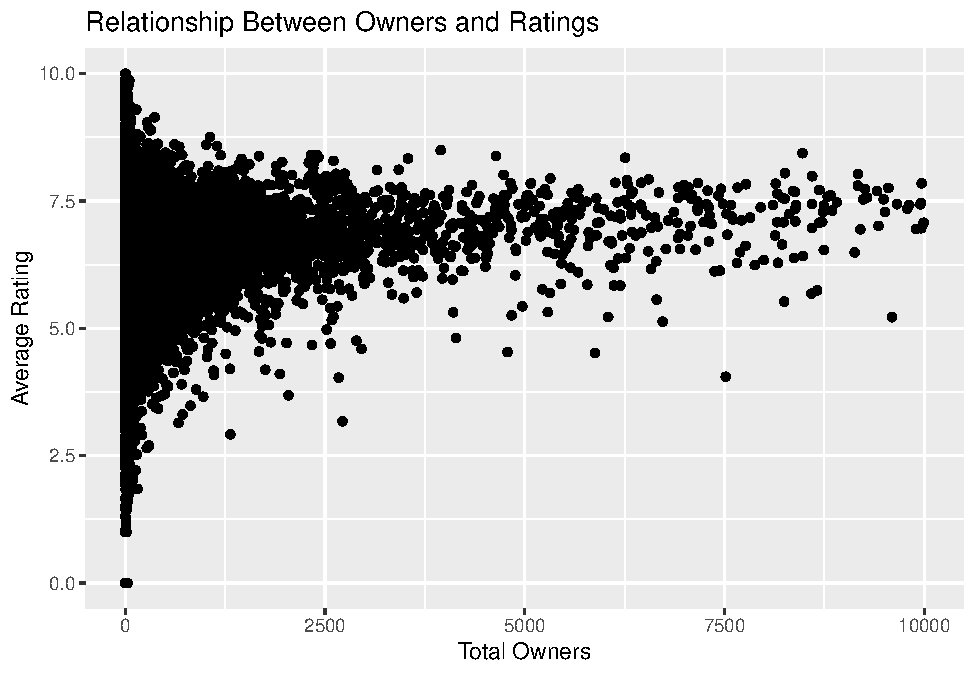
\includegraphics{ANUASS2TEST_files/figure-latex/unnamed-chunk-3-1.pdf}

Considering, for example, the two variable \emph{average\_rating} and
\emph{total\_owners}, the plot above make us see which is the
relationship between them.

\hypertarget{point-b}{%
\subsection{Point b}\label{point-b}}

\begin{Shaded}
\begin{Highlighting}[]
\NormalTok{games }\OtherTok{\textless{}{-}}\NormalTok{ games[,}\SpecialCharTok{{-}}\FunctionTok{c}\NormalTok{(}\DecValTok{1}\NormalTok{,}\DecValTok{2}\NormalTok{)]}
\NormalTok{games }\OtherTok{\textless{}{-}} \FunctionTok{scale}\NormalTok{(games)}
\end{Highlighting}
\end{Shaded}

\begin{Shaded}
\begin{Highlighting}[]
\NormalTok{cov\_matrix }\OtherTok{\textless{}{-}} \FunctionTok{cov}\NormalTok{(games)}
\FunctionTok{ggcorrplot}\NormalTok{(cov\_matrix)}
\end{Highlighting}
\end{Shaded}

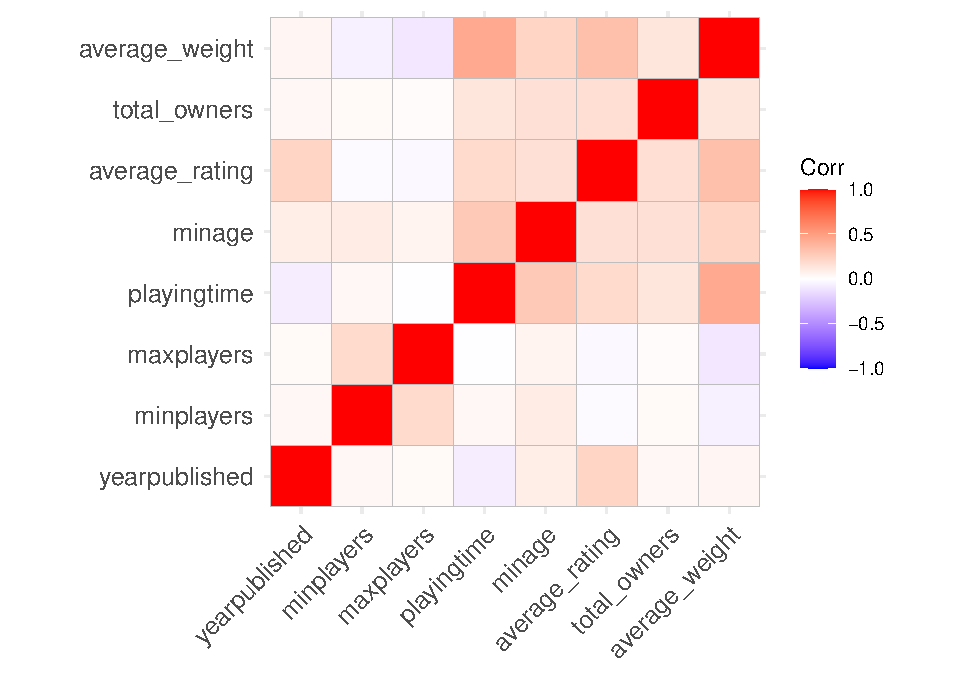
\includegraphics{ANUASS2TEST_files/figure-latex/unnamed-chunk-5-1.pdf}

From the plot and the variance-covariance matrix values we can see that
the variables don't have a strong relationship in general.

\begin{Shaded}
\begin{Highlighting}[]
\NormalTok{cor\_matrix }\OtherTok{\textless{}{-}} \FunctionTok{cor}\NormalTok{(games)}
\FunctionTok{plot}\NormalTok{(cov\_matrix, cor\_matrix, }
     \AttributeTok{xlab =} \StringTok{"Variance{-}Covariance Matrix"}\NormalTok{,}
     \AttributeTok{ylab =} \StringTok{"Correlation Matrix"}\NormalTok{)}
\FunctionTok{abline}\NormalTok{(}\DecValTok{0}\NormalTok{,}\DecValTok{1}\NormalTok{,}\AttributeTok{col =} \StringTok{"red"}\NormalTok{)}
\end{Highlighting}
\end{Shaded}

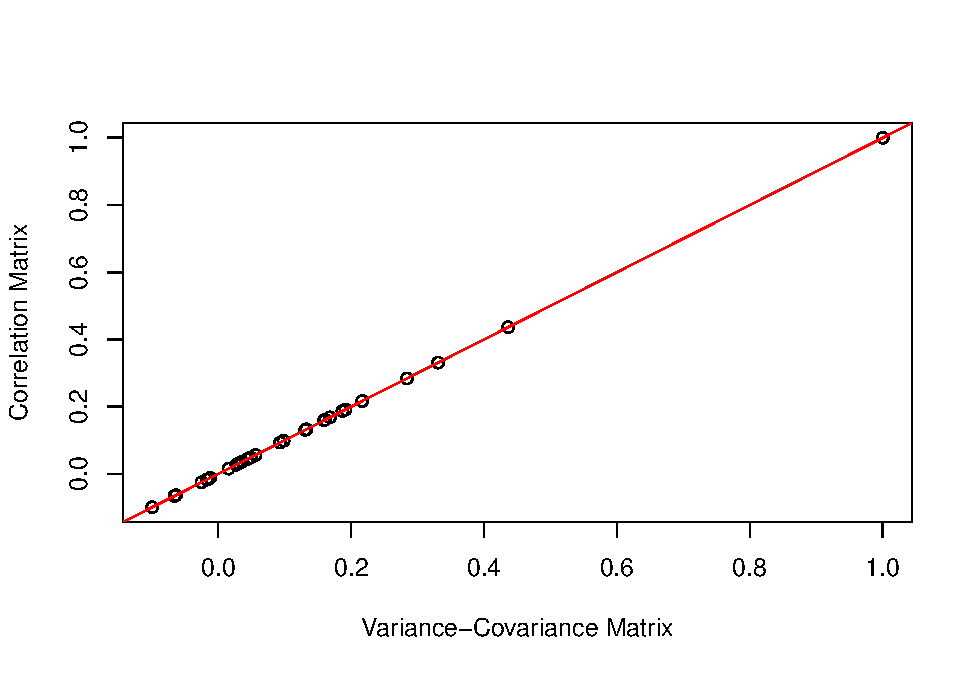
\includegraphics{ANUASS2TEST_files/figure-latex/unnamed-chunk-6-1.pdf}

The correlation matrix is the same as the variance-covariance matrix
because our dataset has been scaled, resulting in equivalent covariance
and correlation values.

\hypertarget{point-c}{%
\subsection{Point c}\label{point-c}}

Now we perform nonparametric bootstrap to obtain standard error
estimates for each of the entries of the variance-covariance matrix.

\begin{Shaded}
\begin{Highlighting}[]
\FunctionTok{set.seed}\NormalTok{(}\DecValTok{12345}\NormalTok{)}

\NormalTok{B }\OtherTok{\textless{}{-}} \DecValTok{1000}
\NormalTok{boot }\OtherTok{\textless{}{-}} \ControlFlowTok{function}\NormalTok{(B, games)\{}
  
\NormalTok{  results }\OtherTok{\textless{}{-}} \FunctionTok{matrix}\NormalTok{(}\ConstantTok{NA}\NormalTok{, }\AttributeTok{nrow =}\NormalTok{ B, }\AttributeTok{ncol =} \FunctionTok{ncol}\NormalTok{(games)}\SpecialCharTok{\^{}}\DecValTok{2}\NormalTok{)}
\NormalTok{  bootstrap }\OtherTok{\textless{}{-}} \FunctionTok{replicate}\NormalTok{(B, \{}
    
\NormalTok{    bootSample }\OtherTok{\textless{}{-}}\NormalTok{ games[}\FunctionTok{sample}\NormalTok{(}\FunctionTok{nrow}\NormalTok{(games), }\AttributeTok{replace =}\NormalTok{ T),]}
\NormalTok{    bootCov }\OtherTok{\textless{}{-}} \FunctionTok{cov}\NormalTok{(bootSample)}
\NormalTok{    i }\OtherTok{\textless{}{-}} \FunctionTok{seq\_len}\NormalTok{(B)}
\NormalTok{    results[i,] }\OtherTok{\textless{}{-}} \FunctionTok{as.vector}\NormalTok{(bootCov)}
\NormalTok{  \})}
  \FunctionTok{return}\NormalTok{(bootstrap)}
\NormalTok{\}}

\NormalTok{boot }\OtherTok{\textless{}{-}} \FunctionTok{boot}\NormalTok{(}\DecValTok{1000}\NormalTok{,games)}

\NormalTok{standard\_errors }\OtherTok{\textless{}{-}} \FunctionTok{apply}\NormalTok{(boot, }\DecValTok{1}\NormalTok{, sd)}
\NormalTok{standard\_errors}
\end{Highlighting}
\end{Shaded}

\begin{verbatim}
##  [1] 0.016767571 0.005726342 0.005392461 0.006026930 0.006611704 0.006527865
##  [7] 0.006366352 0.006391746 0.005726342 0.030878533 0.012807945 0.008199441
## [13] 0.007928323 0.006332489 0.007044940 0.006013313 0.005392461 0.012807945
## [19] 0.082934774 0.005253855 0.006605301 0.005991273 0.004863436 0.005935743
## [25] 0.006026930 0.008199441 0.005253855 0.012317292 0.006937599 0.006049556
## [31] 0.006927497 0.007735376 0.006611704 0.007928323 0.006605301 0.006937599
## [37] 0.018955155 0.007341887 0.004957443 0.007548761 0.006527865 0.006332489
## [43] 0.005991273 0.006049556 0.007341887 0.015166272 0.005447973 0.007162792
## [49] 0.006366352 0.007044940 0.004863436 0.006927497 0.004957443 0.005447973
## [55] 0.044025974 0.006719733 0.006391746 0.006013313 0.005935743 0.007735376
## [61] 0.007548761 0.007162792 0.006719733 0.010072221
\end{verbatim}

Now we obtain confidence intervals of the bootstrap distribution using
the percentile approach and the central limit theorem (CLT).

\begin{Shaded}
\begin{Highlighting}[]
\NormalTok{means }\OtherTok{\textless{}{-}} \FunctionTok{apply}\NormalTok{(boot, }\DecValTok{1}\NormalTok{, mean)}
\NormalTok{qnt\_CI }\OtherTok{\textless{}{-}} \FunctionTok{t}\NormalTok{(}\FunctionTok{apply}\NormalTok{(boot, }\DecValTok{1}\NormalTok{, }\ControlFlowTok{function}\NormalTok{(z) }\FunctionTok{quantile}\NormalTok{(z, }\AttributeTok{probs =} \FunctionTok{c}\NormalTok{(}\FloatTok{0.025}\NormalTok{,}\FloatTok{0.975}\NormalTok{))))}
\NormalTok{clt\_CI }\OtherTok{\textless{}{-}}\NormalTok{ means }\SpecialCharTok{+} \FunctionTok{c}\NormalTok{(}\SpecialCharTok{{-}}\DecValTok{1}\NormalTok{,}\DecValTok{1}\NormalTok{)}\SpecialCharTok{*}\FloatTok{1.96}\SpecialCharTok{*}\NormalTok{standard\_errors}
\NormalTok{cov\_hat }\OtherTok{\textless{}{-}} \FunctionTok{as.vector}\NormalTok{(cov\_matrix)}
\NormalTok{x }\OtherTok{\textless{}{-}} \FunctionTok{seq}\NormalTok{(}\FunctionTok{length}\NormalTok{(cov\_hat))}
\NormalTok{y }\OtherTok{\textless{}{-}}\NormalTok{ cov\_hat}
\NormalTok{y\_upper }\OtherTok{\textless{}{-}} \FunctionTok{unlist}\NormalTok{(qnt\_CI[,}\DecValTok{2}\NormalTok{])}
\NormalTok{y\_lower }\OtherTok{\textless{}{-}} \FunctionTok{unlist}\NormalTok{(qnt\_CI[,}\DecValTok{1}\NormalTok{])}
\FunctionTok{plot}\NormalTok{(y, }\AttributeTok{pch =} \DecValTok{19}\NormalTok{, }\AttributeTok{cex =} \FloatTok{0.5}\NormalTok{,}\AttributeTok{ylim =} \FunctionTok{range}\NormalTok{(}\FunctionTok{c}\NormalTok{(y\_lower, y\_upper)), }\AttributeTok{ylab =} \StringTok{"Var/Cov"}\NormalTok{, }\AttributeTok{xlab =} \StringTok{"Index"}\NormalTok{,}
     \AttributeTok{main =} \StringTok{"Percentile Approach Confidence Intervals"}\NormalTok{)}
\FunctionTok{segments}\NormalTok{(x, y\_lower, x, y\_upper, }\AttributeTok{lwd =} \FloatTok{1.5}\NormalTok{,}\AttributeTok{col =} \StringTok{"blue"}\NormalTok{)}
\end{Highlighting}
\end{Shaded}

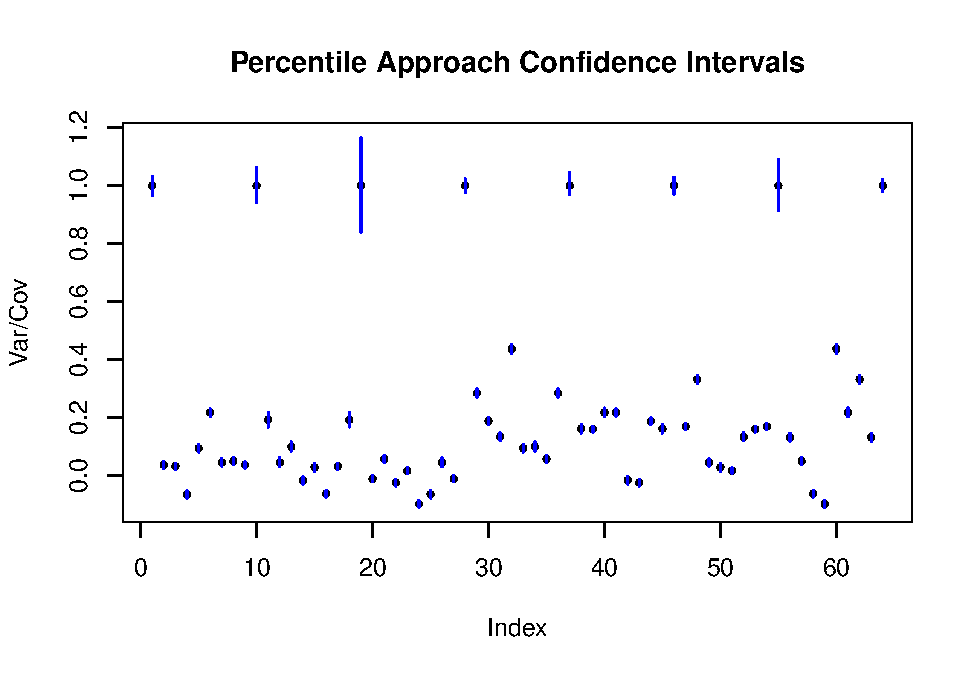
\includegraphics{ANUASS2TEST_files/figure-latex/unnamed-chunk-8-1.pdf}

Above there is the plot of the confidence intervals of each entry of the
variance-covariance matrix (Index) using the percentile approach.

\begin{Shaded}
\begin{Highlighting}[]
\FunctionTok{plot}\NormalTok{(}\DecValTok{1}\SpecialCharTok{:}\FunctionTok{length}\NormalTok{(standard\_errors), standard\_errors, }\AttributeTok{type =} \StringTok{"l"}\NormalTok{, }
     \AttributeTok{xlab =} \StringTok{"Bootstrap Iterations"}\NormalTok{, }\AttributeTok{ylab =} \StringTok{"Standard Error"}\NormalTok{, }
     \AttributeTok{main =} \StringTok{"Standard Errors of Bootstrap Estimates"}\NormalTok{)}
\end{Highlighting}
\end{Shaded}

\includegraphics{ANUASS2TEST_files/figure-latex/unnamed-chunk-9-1.pdf}

\hypertarget{point-d}{%
\subsection{Point d}\label{point-d}}

Show the behavior of the values \(\{\theta_j\}_{j=1}^p\) and estimate
\(j^*\).

\begin{Shaded}
\begin{Highlighting}[]
\NormalTok{eigen\_values }\OtherTok{\textless{}{-}} \FunctionTok{eigen}\NormalTok{(cov\_matrix)}\SpecialCharTok{$}\NormalTok{values}
\NormalTok{theta }\OtherTok{\textless{}{-}} \FunctionTok{cumsum}\NormalTok{(eigen\_values) }\SpecialCharTok{/} \FunctionTok{sum}\NormalTok{(eigen\_values)}
\NormalTok{theta}
\end{Highlighting}
\end{Shaded}

\begin{verbatim}
## [1] 0.2426729 0.4008816 0.5410761 0.6550491 0.7568552 0.8551548 0.9359288
## [8] 1.0000000
\end{verbatim}

\begin{Shaded}
\begin{Highlighting}[]
\NormalTok{jstar }\OtherTok{\textless{}{-}} \FunctionTok{min}\NormalTok{(}\FunctionTok{which}\NormalTok{(theta }\SpecialCharTok{\textgreater{}} \FloatTok{0.76}\NormalTok{))}
\NormalTok{jstar}
\end{Highlighting}
\end{Shaded}

\begin{verbatim}
## [1] 6
\end{verbatim}

\hypertarget{point-e}{%
\subsection{Point e}\label{point-e}}

Perform bootstrap to estimate the bias and standard error of the
estimators for the parameters in the sequence \(\{\theta_j\}_{j=1}^p\).

\begin{Shaded}
\begin{Highlighting}[]
\NormalTok{boot\_theta }\OtherTok{\textless{}{-}} \FunctionTok{matrix}\NormalTok{(}\DecValTok{0}\NormalTok{, }\AttributeTok{nrow =}\NormalTok{ B, }\AttributeTok{ncol =} \FunctionTok{length}\NormalTok{(theta))}
\NormalTok{boot\_jstar }\OtherTok{\textless{}{-}} \FunctionTok{numeric}\NormalTok{(B)}
\ControlFlowTok{for}\NormalTok{ (i }\ControlFlowTok{in} \DecValTok{1}\SpecialCharTok{:}\NormalTok{B) \{}
\NormalTok{  boot\_sample }\OtherTok{\textless{}{-}}\NormalTok{ games[}\FunctionTok{sample}\NormalTok{(}\FunctionTok{nrow}\NormalTok{(games), }\AttributeTok{replace=} \ConstantTok{TRUE}\NormalTok{),]}
\NormalTok{  cov\_boot }\OtherTok{\textless{}{-}} \FunctionTok{cov}\NormalTok{(boot\_sample)}
\NormalTok{  eigen\_boot }\OtherTok{\textless{}{-}} \FunctionTok{eigen}\NormalTok{(cov\_boot)}\SpecialCharTok{$}\NormalTok{values}
\NormalTok{  boot\_theta[i,] }\OtherTok{\textless{}{-}} \FunctionTok{cumsum}\NormalTok{(eigen\_boot) }\SpecialCharTok{/} \FunctionTok{sum}\NormalTok{(eigen\_boot)}
\NormalTok{  boot\_jstar[i] }\OtherTok{\textless{}{-}} \FunctionTok{min}\NormalTok{(}\FunctionTok{which}\NormalTok{(boot\_theta[i,] }\SpecialCharTok{\textgreater{}} \FloatTok{0.76}\NormalTok{))}
\NormalTok{\}}
\end{Highlighting}
\end{Shaded}

\begin{Shaded}
\begin{Highlighting}[]
\NormalTok{bias }\OtherTok{\textless{}{-}} \FunctionTok{colMeans}\NormalTok{(boot\_theta)}\SpecialCharTok{{-}}\NormalTok{theta}
\NormalTok{se }\OtherTok{\textless{}{-}} \FunctionTok{apply}\NormalTok{(boot\_theta, }\DecValTok{2}\NormalTok{, sd)}
\NormalTok{bias}
\end{Highlighting}
\end{Shaded}

\begin{verbatim}
## [1] 2.660301e-04 8.058590e-04 7.381508e-04 9.166828e-04 1.767983e-03
## [6] 2.008943e-04 9.475436e-05 0.000000e+00
\end{verbatim}

\begin{Shaded}
\begin{Highlighting}[]
\NormalTok{se}
\end{Highlighting}
\end{Shaded}

\begin{verbatim}
## [1] 0.003174574 0.002647125 0.002873812 0.003279194 0.002552820 0.002106016
## [7] 0.001101662 0.000000000
\end{verbatim}

Also report the bootstrap estimates and standard errors for the
estimator of \(j^*\).

\begin{Shaded}
\begin{Highlighting}[]
\NormalTok{bias\_jstar }\OtherTok{\textless{}{-}} \FunctionTok{mean}\NormalTok{(boot\_jstar) }\SpecialCharTok{{-}}\NormalTok{ jstar}
\NormalTok{se\_jstar }\OtherTok{\textless{}{-}} \FunctionTok{sd}\NormalTok{(boot\_jstar)}
\NormalTok{bias\_jstar}
\end{Highlighting}
\end{Shaded}

\begin{verbatim}
## [1] -0.278
\end{verbatim}

\begin{Shaded}
\begin{Highlighting}[]
\NormalTok{se\_jstar}
\end{Highlighting}
\end{Shaded}

\begin{verbatim}
## [1] 0.4482376
\end{verbatim}

Finally, give an estimate for \(P(\hat{j^*=5})\).

\begin{Shaded}
\begin{Highlighting}[]
\NormalTok{p\_jstar }\OtherTok{\textless{}{-}} \FunctionTok{mean}\NormalTok{(boot\_jstar}\SpecialCharTok{==}\DecValTok{5}\NormalTok{)}
\NormalTok{p\_jstar}
\end{Highlighting}
\end{Shaded}

\begin{verbatim}
## [1] 0.278
\end{verbatim}

\hypertarget{point-f}{%
\subsection{Point f}\label{point-f}}

Run a linear regression with average\_rating as target variable,
regressed over all the other variables.

\begin{Shaded}
\begin{Highlighting}[]
\FunctionTok{set.seed}\NormalTok{(}\FunctionTok{abs}\NormalTok{(}\DecValTok{636{-}555{-}3226}\NormalTok{))}
\NormalTok{ind }\OtherTok{\textless{}{-}} \FunctionTok{sample}\NormalTok{(}\DecValTok{1}\SpecialCharTok{:}\FunctionTok{nrow}\NormalTok{(games),}\DecValTok{5000}\NormalTok{,}\ConstantTok{FALSE}\NormalTok{)}
\NormalTok{sub\_data }\OtherTok{\textless{}{-}}\NormalTok{ games[ind,]}

\NormalTok{sub\_data }\OtherTok{\textless{}{-}} \FunctionTok{as.data.frame}\NormalTok{(sub\_data)}
\NormalTok{regression }\OtherTok{\textless{}{-}} \FunctionTok{lm}\NormalTok{(sub\_data}\SpecialCharTok{$}\NormalTok{average\_rating}\SpecialCharTok{\textasciitilde{}}\NormalTok{., }\AttributeTok{data =}\NormalTok{ sub\_data)}
\FunctionTok{summary}\NormalTok{(regression)  }
\end{Highlighting}
\end{Shaded}

\begin{verbatim}
## 
## Call:
## lm(formula = sub_data$average_rating ~ ., data = sub_data)
## 
## Residuals:
##     Min      1Q  Median      3Q     Max 
## -4.9202 -0.3275  0.0989  0.4873  3.1911 
## 
## Coefficients:
##                 Estimate Std. Error t value Pr(>|t|)    
## (Intercept)     0.008392   0.012916   0.650  0.51587    
## yearpublished   0.199808   0.013454  14.851  < 2e-16 ***
## minplayers     -0.010653   0.013532  -0.787  0.43119    
## maxplayers     -0.006019   0.013517  -0.445  0.65614    
## playingtime     0.077747   0.014689   5.293 1.26e-07 ***
## minage          0.041984   0.013271   3.164  0.00157 ** 
## total_owners    0.111174   0.013423   8.283  < 2e-16 ***
## average_weight  0.228837   0.014440  15.848  < 2e-16 ***
## ---
## Signif. codes:  0 '***' 0.001 '**' 0.01 '*' 0.05 '.' 0.1 ' ' 1
## 
## Residual standard error: 0.9129 on 4992 degrees of freedom
## Multiple R-squared:  0.151,  Adjusted R-squared:  0.1498 
## F-statistic: 126.9 on 7 and 4992 DF,  p-value: < 2.2e-16
\end{verbatim}

The intercept is equal to 0.008392. It corresponds to the expected
average rate of a board game when the other variables are equal to zero.
And so it is not interpretable in this problem because we are talking
about the average rating of a board game that does not exist. We can use
the \(R^2\) to assess the goodness of fit of our linear regression
model, that is equal to 0.151. It means that only 15,1\% of the the
variation in \emph{average\_rating} is explained by the regressors.

\hypertarget{point-g}{%
\subsection{Point g}\label{point-g}}

\begin{Shaded}
\begin{Highlighting}[]
\FunctionTok{plot}\NormalTok{(}\FunctionTok{fitted}\NormalTok{(regression), }\FunctionTok{resid}\NormalTok{(regression))}
\FunctionTok{abline}\NormalTok{(}\DecValTok{0}\NormalTok{,}\DecValTok{0}\NormalTok{,}\AttributeTok{col =} \StringTok{"red"}\NormalTok{)}
\end{Highlighting}
\end{Shaded}

\includegraphics{ANUASS2TEST_files/figure-latex/unnamed-chunk-17-1.pdf}

Below we used the paired bootstrap method to provide bias, standard
error and confidence intervals for regression coefficients, adjusted
\(R^2\) index and our \(\hat{\theta}\). In particular, we chose this
method and, for example, not the bootstrap of the errors because in the
plot above it is possible to see that the residuals seem to not have
constant variance.

\begin{Shaded}
\begin{Highlighting}[]
\FunctionTok{set.seed}\NormalTok{(}\FunctionTok{abs}\NormalTok{(}\DecValTok{636{-}555{-}3226}\NormalTok{))}
\NormalTok{perform\_paired\_bootstrap }\OtherTok{\textless{}{-}} \ControlFlowTok{function}\NormalTok{(data, B) \{}
\NormalTok{  num\_coeffs }\OtherTok{\textless{}{-}} \FunctionTok{length}\NormalTok{(}\FunctionTok{coef}\NormalTok{(regression))}
\NormalTok{  bootstrap\_estimates }\OtherTok{\textless{}{-}} \FunctionTok{matrix}\NormalTok{(}\DecValTok{0}\NormalTok{, }\AttributeTok{nrow =}\NormalTok{ B, }\AttributeTok{ncol =}\NormalTok{ num\_coeffs)}
  
  \ControlFlowTok{for}\NormalTok{ (i }\ControlFlowTok{in} \DecValTok{1}\SpecialCharTok{:}\NormalTok{B) \{}
\NormalTok{    bootstrap\_indices }\OtherTok{\textless{}{-}} \FunctionTok{sample}\NormalTok{(}\FunctionTok{nrow}\NormalTok{(data), }\AttributeTok{replace =} \ConstantTok{TRUE}\NormalTok{)}
\NormalTok{    bootstrap\_sample }\OtherTok{\textless{}{-}}\NormalTok{ data[bootstrap\_indices, ]}
\NormalTok{    bootstrap\_regression }\OtherTok{\textless{}{-}} \FunctionTok{lm}\NormalTok{(average\_rating }\SpecialCharTok{\textasciitilde{}}\NormalTok{ ., }\AttributeTok{data =}\NormalTok{ bootstrap\_sample)}
\NormalTok{    bootstrap\_estimates[i, ] }\OtherTok{\textless{}{-}} \FunctionTok{coef}\NormalTok{(bootstrap\_regression)}
\NormalTok{  \}}
  
\NormalTok{  coefficient\_bias }\OtherTok{\textless{}{-}} \FunctionTok{apply}\NormalTok{(bootstrap\_estimates, }\DecValTok{2}\NormalTok{, mean) }\SpecialCharTok{{-}} \FunctionTok{coef}\NormalTok{(regression)}
\NormalTok{  coefficient\_std\_error }\OtherTok{\textless{}{-}} \FunctionTok{apply}\NormalTok{(bootstrap\_estimates, }\DecValTok{2}\NormalTok{, sd)}
\NormalTok{  coefficient\_confidence\_intervals }\OtherTok{\textless{}{-}} \FunctionTok{t}\NormalTok{(}\FunctionTok{apply}\NormalTok{(bootstrap\_estimates, }\DecValTok{2}\NormalTok{, }\ControlFlowTok{function}\NormalTok{(x) }\FunctionTok{quantile}\NormalTok{(x, }\FunctionTok{c}\NormalTok{(}\FloatTok{0.025}\NormalTok{, }\FloatTok{0.975}\NormalTok{))))}
  
\NormalTok{  adjusted\_r\_squared }\OtherTok{\textless{}{-}} \FunctionTok{numeric}\NormalTok{(B)}
  \ControlFlowTok{for}\NormalTok{ (i }\ControlFlowTok{in} \DecValTok{1}\SpecialCharTok{:}\NormalTok{B) \{}
\NormalTok{    bootstrap\_indices }\OtherTok{\textless{}{-}} \FunctionTok{sample}\NormalTok{(}\FunctionTok{nrow}\NormalTok{(data), }\AttributeTok{replace =} \ConstantTok{TRUE}\NormalTok{)}
\NormalTok{    bootstrap\_sample }\OtherTok{\textless{}{-}}\NormalTok{ data[bootstrap\_indices, ]}
\NormalTok{    bootstrap\_regression }\OtherTok{\textless{}{-}} \FunctionTok{lm}\NormalTok{(average\_rating }\SpecialCharTok{\textasciitilde{}}\NormalTok{ ., }\AttributeTok{data =}\NormalTok{ bootstrap\_sample)}
\NormalTok{    adjusted\_r\_squared[i] }\OtherTok{\textless{}{-}} \DecValTok{1} \SpecialCharTok{{-}}\NormalTok{ (}\DecValTok{1} \SpecialCharTok{{-}} \FunctionTok{summary}\NormalTok{(bootstrap\_regression)}\SpecialCharTok{$}\NormalTok{r.squared) }\SpecialCharTok{*}\NormalTok{ ((}\FunctionTok{nrow}\NormalTok{(bootstrap\_sample) }\SpecialCharTok{{-}} \DecValTok{1}\NormalTok{) }\SpecialCharTok{/}\NormalTok{ (}\FunctionTok{nrow}\NormalTok{(bootstrap\_sample) }\SpecialCharTok{{-}} \FunctionTok{length}\NormalTok{(}\FunctionTok{coef}\NormalTok{(bootstrap\_regression)) }\SpecialCharTok{{-}} \DecValTok{1}\NormalTok{))}
\NormalTok{  \}}
\NormalTok{  adjusted\_r\_squared\_bias }\OtherTok{\textless{}{-}} \FunctionTok{mean}\NormalTok{(adjusted\_r\_squared) }\SpecialCharTok{{-}} \FunctionTok{summary}\NormalTok{(regression)}\SpecialCharTok{$}\NormalTok{adj.r.squared}
\NormalTok{  adjusted\_r\_squared\_std\_error }\OtherTok{\textless{}{-}} \FunctionTok{sd}\NormalTok{(adjusted\_r\_squared)}
\NormalTok{  adjusted\_r\_squared\_confidence\_interval }\OtherTok{\textless{}{-}} \FunctionTok{quantile}\NormalTok{(adjusted\_r\_squared, }\FunctionTok{c}\NormalTok{(}\FloatTok{0.025}\NormalTok{, }\FloatTok{0.975}\NormalTok{))}
  
\NormalTok{  theta\_estimates }\OtherTok{\textless{}{-}} \FunctionTok{numeric}\NormalTok{(B)}
\NormalTok{  coeff }\OtherTok{\textless{}{-}} \FunctionTok{coef}\NormalTok{(regression)}
  
  \ControlFlowTok{for}\NormalTok{ (i }\ControlFlowTok{in} \DecValTok{1}\SpecialCharTok{:}\NormalTok{B) \{}
\NormalTok{    boot\_sample }\OtherTok{\textless{}{-}}\NormalTok{ data[}\FunctionTok{sample}\NormalTok{(}\FunctionTok{nrow}\NormalTok{(data), }\AttributeTok{replace =} \ConstantTok{TRUE}\NormalTok{), ]}
\NormalTok{    regression\_boot }\OtherTok{\textless{}{-}} \FunctionTok{lm}\NormalTok{(average\_rating }\SpecialCharTok{\textasciitilde{}}\NormalTok{ ., }\AttributeTok{data =}\NormalTok{ boot\_sample)}
\NormalTok{    coeff\_boot }\OtherTok{\textless{}{-}} \FunctionTok{coef}\NormalTok{(regression\_boot)}
\NormalTok{    theta\_boot }\OtherTok{\textless{}{-}} \FunctionTok{max}\NormalTok{(((coeff\_boot[}\DecValTok{5}\NormalTok{] }\SpecialCharTok{{-}}\NormalTok{ coeff\_boot[}\DecValTok{6}\NormalTok{])}\SpecialCharTok{/}\NormalTok{(coeff\_boot[}\DecValTok{3}\NormalTok{]}\SpecialCharTok{+}\NormalTok{coeff\_boot[}\DecValTok{2}\NormalTok{])), }\DecValTok{0}\NormalTok{)}
\NormalTok{    theta\_estimates[i] }\OtherTok{\textless{}{-}}\NormalTok{ theta\_boot}
\NormalTok{  \}}
  
\NormalTok{  bias }\OtherTok{\textless{}{-}} \FunctionTok{mean}\NormalTok{(theta\_estimates) }\SpecialCharTok{{-}}\NormalTok{ ((coeff[}\DecValTok{5}\NormalTok{] }\SpecialCharTok{{-}}\NormalTok{ coeff[}\DecValTok{6}\NormalTok{])}\SpecialCharTok{/}\NormalTok{(coeff[}\DecValTok{3}\NormalTok{]}\SpecialCharTok{+}\NormalTok{coeff[}\DecValTok{2}\NormalTok{]))}
\NormalTok{  se }\OtherTok{\textless{}{-}} \FunctionTok{sd}\NormalTok{(theta\_estimates)}
\NormalTok{  ci }\OtherTok{\textless{}{-}} \FunctionTok{quantile}\NormalTok{(theta\_estimates, }\AttributeTok{probs =} \FunctionTok{c}\NormalTok{(}\FloatTok{0.025}\NormalTok{, }\FloatTok{0.975}\NormalTok{))}
  
\NormalTok{  results }\OtherTok{\textless{}{-}} \FunctionTok{list}\NormalTok{(}
    \AttributeTok{coefficient\_bias =}\NormalTok{ coefficient\_bias,}
    \AttributeTok{coefficient\_std\_error =}\NormalTok{ coefficient\_std\_error,}
    \AttributeTok{coefficient\_confidence\_intervals =}\NormalTok{ coefficient\_confidence\_intervals,}
    \AttributeTok{adjusted\_r\_squared\_bias =}\NormalTok{ adjusted\_r\_squared\_bias,}
    \AttributeTok{adjusted\_r\_squared\_std\_error =}\NormalTok{ adjusted\_r\_squared\_std\_error,}
    \AttributeTok{adjusted\_r\_squared\_confidence\_interval =}\NormalTok{ adjusted\_r\_squared\_confidence\_interval,}
    \AttributeTok{theta\_bias =}\NormalTok{ bias,}
    \AttributeTok{theta\_std\_error =}\NormalTok{ se,}
    \AttributeTok{theta\_confidence\_interval =}\NormalTok{ ci}
\NormalTok{  )}
  
  \FunctionTok{return}\NormalTok{(results)}
\NormalTok{\}}

\NormalTok{results }\OtherTok{\textless{}{-}} \FunctionTok{perform\_paired\_bootstrap}\NormalTok{(sub\_data, B)}
\NormalTok{results}
\end{Highlighting}
\end{Shaded}

\begin{verbatim}
## $coefficient_bias
##    (Intercept)  yearpublished     minplayers     maxplayers    playingtime 
##   2.590343e-04  -5.313236e-04   5.391762e-05  -3.615397e-04  -2.715688e-04 
##         minage   total_owners average_weight 
##  -9.566880e-05   4.931990e-04  -6.421485e-05 
## 
## $coefficient_std_error
## [1] 0.012917019 0.014882237 0.014706065 0.009575085 0.013402492 0.013637539
## [7] 0.007677498 0.017932378
## 
## $coefficient_confidence_intervals
##             2.5%      97.5%
## [1,] -0.01545676 0.03319964
## [2,]  0.17137553 0.22927323
## [3,] -0.03924184 0.01808103
## [4,] -0.02516037 0.01208000
## [5,]  0.05100863 0.10383718
## [6,]  0.01570397 0.06778159
## [7,]  0.09695728 0.12696910
## [8,]  0.19381726 0.26420035
## 
## $adjusted_r_squared_bias
## [1] 0.0005191378
## 
## $adjusted_r_squared_std_error
## [1] 0.01122473
## 
## $adjusted_r_squared_confidence_interval
##      2.5%     97.5% 
## 0.1292476 0.1717044 
## 
## $theta_bias
## playingtime 
## 0.008709073 
## 
## $theta_std_error
## [1] 0.1101246
## 
## $theta_confidence_interval
##      2.5%     97.5% 
## 0.0000000 0.4221232
\end{verbatim}

\hypertarget{point-h}{%
\subsection{Point h}\label{point-h}}

\begin{Shaded}
\begin{Highlighting}[]
\FunctionTok{set.seed}\NormalTok{(}\FunctionTok{abs}\NormalTok{(}\DecValTok{636{-}555{-}3226}\NormalTok{))}
\NormalTok{perform\_jackknife }\OtherTok{\textless{}{-}} \ControlFlowTok{function}\NormalTok{(data) \{}
\NormalTok{  num\_coeffs }\OtherTok{\textless{}{-}} \FunctionTok{length}\NormalTok{(}\FunctionTok{coef}\NormalTok{(regression))}
\NormalTok{  num\_samples }\OtherTok{\textless{}{-}} \FunctionTok{nrow}\NormalTok{(data)}
\NormalTok{  jackknife\_estimates }\OtherTok{\textless{}{-}} \FunctionTok{matrix}\NormalTok{(}\DecValTok{0}\NormalTok{, }\AttributeTok{nrow =}\NormalTok{ num\_samples, }\AttributeTok{ncol =}\NormalTok{ num\_coeffs)}
  
  \ControlFlowTok{for}\NormalTok{ (i }\ControlFlowTok{in} \DecValTok{1}\SpecialCharTok{:}\NormalTok{num\_samples) \{}
\NormalTok{    jackknife\_sample }\OtherTok{\textless{}{-}}\NormalTok{ data[}\SpecialCharTok{{-}}\NormalTok{i, ] }
\NormalTok{    jackknife\_regression }\OtherTok{\textless{}{-}} \FunctionTok{lm}\NormalTok{(average\_rating }\SpecialCharTok{\textasciitilde{}}\NormalTok{ ., }\AttributeTok{data =}\NormalTok{ jackknife\_sample)}
\NormalTok{    jackknife\_estimates[i, ] }\OtherTok{\textless{}{-}} \FunctionTok{coef}\NormalTok{(jackknife\_regression)}
\NormalTok{  \}}
  
\NormalTok{  coefficient\_bias }\OtherTok{\textless{}{-}}\NormalTok{ num\_samples }\SpecialCharTok{*}\NormalTok{ (}\FunctionTok{colMeans}\NormalTok{(jackknife\_estimates) }\SpecialCharTok{{-}} \FunctionTok{coef}\NormalTok{(regression)) }\SpecialCharTok{/}\NormalTok{ (num\_samples }\SpecialCharTok{{-}} \DecValTok{1}\NormalTok{)}
\NormalTok{  coefficient\_std\_error }\OtherTok{\textless{}{-}} \FunctionTok{sqrt}\NormalTok{(num\_samples }\SpecialCharTok{*}\NormalTok{ (}\FunctionTok{colMeans}\NormalTok{(jackknife\_estimates}\SpecialCharTok{\^{}}\DecValTok{2}\NormalTok{) }\SpecialCharTok{{-}}\NormalTok{ (}\FunctionTok{colMeans}\NormalTok{(jackknife\_estimates))}\SpecialCharTok{\^{}}\DecValTok{2}\NormalTok{) }\SpecialCharTok{/}\NormalTok{ (num\_samples }\SpecialCharTok{{-}} \DecValTok{1}\NormalTok{))}
\NormalTok{  coefficient\_confidence\_intervals }\OtherTok{\textless{}{-}} \FunctionTok{t}\NormalTok{(}\FunctionTok{apply}\NormalTok{(jackknife\_estimates, }\DecValTok{2}\NormalTok{, }\ControlFlowTok{function}\NormalTok{(x) }\FunctionTok{quantile}\NormalTok{(x, }\FunctionTok{c}\NormalTok{(}\FloatTok{0.025}\NormalTok{, }\FloatTok{0.975}\NormalTok{))))}
  
\NormalTok{  adjusted\_r\_squared }\OtherTok{\textless{}{-}} \FunctionTok{numeric}\NormalTok{(num\_samples)}
  \ControlFlowTok{for}\NormalTok{ (i }\ControlFlowTok{in} \DecValTok{1}\SpecialCharTok{:}\NormalTok{num\_samples) \{}
\NormalTok{    jackknife\_sample }\OtherTok{\textless{}{-}}\NormalTok{ data[}\SpecialCharTok{{-}}\NormalTok{i, ]}
\NormalTok{    jackknife\_regression }\OtherTok{\textless{}{-}} \FunctionTok{lm}\NormalTok{(average\_rating }\SpecialCharTok{\textasciitilde{}}\NormalTok{ ., }\AttributeTok{data =}\NormalTok{ jackknife\_sample)}
\NormalTok{    adjusted\_r\_squared[i] }\OtherTok{\textless{}{-}} \DecValTok{1} \SpecialCharTok{{-}}\NormalTok{ (}\DecValTok{1} \SpecialCharTok{{-}} \FunctionTok{summary}\NormalTok{(jackknife\_regression)}\SpecialCharTok{$}\NormalTok{r.squared) }\SpecialCharTok{*}\NormalTok{ ((}\FunctionTok{nrow}\NormalTok{(jackknife\_sample) }\SpecialCharTok{{-}} \DecValTok{1}\NormalTok{) }\SpecialCharTok{/}\NormalTok{ (}\FunctionTok{nrow}\NormalTok{(jackknife\_sample) }\SpecialCharTok{{-}} \FunctionTok{length}\NormalTok{(}\FunctionTok{coef}\NormalTok{(jackknife\_regression)) }\SpecialCharTok{{-}} \DecValTok{1}\NormalTok{))}
\NormalTok{  \}}
\NormalTok{  adjusted\_r\_squared\_bias }\OtherTok{\textless{}{-}}\NormalTok{ num\_samples }\SpecialCharTok{*}\NormalTok{ (}\FunctionTok{mean}\NormalTok{(adjusted\_r\_squared) }\SpecialCharTok{{-}} \FunctionTok{summary}\NormalTok{(regression)}\SpecialCharTok{$}\NormalTok{adj.r.squared) }\SpecialCharTok{/}\NormalTok{ (num\_samples }\SpecialCharTok{{-}} \DecValTok{1}\NormalTok{)}
\NormalTok{  adjusted\_r\_squared\_std\_error }\OtherTok{\textless{}{-}} \FunctionTok{sqrt}\NormalTok{(num\_samples }\SpecialCharTok{*}\NormalTok{ (}\FunctionTok{mean}\NormalTok{(adjusted\_r\_squared}\SpecialCharTok{\^{}}\DecValTok{2}\NormalTok{) }\SpecialCharTok{{-}}\NormalTok{ (}\FunctionTok{mean}\NormalTok{(adjusted\_r\_squared))}\SpecialCharTok{\^{}}\DecValTok{2}\NormalTok{) }\SpecialCharTok{/}\NormalTok{ (num\_samples }\SpecialCharTok{{-}} \DecValTok{1}\NormalTok{))}
\NormalTok{  adjusted\_r\_squared\_confidence\_interval }\OtherTok{\textless{}{-}} \FunctionTok{quantile}\NormalTok{(adjusted\_r\_squared, }\FunctionTok{c}\NormalTok{(}\FloatTok{0.025}\NormalTok{, }\FloatTok{0.975}\NormalTok{))}
  
\NormalTok{  theta\_estimates }\OtherTok{\textless{}{-}} \FunctionTok{numeric}\NormalTok{(num\_samples)}
\NormalTok{  coeff }\OtherTok{\textless{}{-}} \FunctionTok{coef}\NormalTok{(regression)}
  
  \ControlFlowTok{for}\NormalTok{ (i }\ControlFlowTok{in} \DecValTok{1}\SpecialCharTok{:}\NormalTok{num\_samples) \{}
\NormalTok{    jackknife\_sample }\OtherTok{\textless{}{-}}\NormalTok{ data[}\SpecialCharTok{{-}}\NormalTok{i, ]}
\NormalTok{    jackknife\_regression }\OtherTok{\textless{}{-}} \FunctionTok{lm}\NormalTok{(average\_rating }\SpecialCharTok{\textasciitilde{}}\NormalTok{ ., }\AttributeTok{data =}\NormalTok{ jackknife\_sample)}
\NormalTok{    coeff\_boot }\OtherTok{\textless{}{-}} \FunctionTok{coef}\NormalTok{(jackknife\_regression)}
\NormalTok{    theta\_estimates[i] }\OtherTok{\textless{}{-}} \FunctionTok{max}\NormalTok{(((coeff\_boot[}\DecValTok{5}\NormalTok{] }\SpecialCharTok{{-}}\NormalTok{ coeff\_boot[}\DecValTok{6}\NormalTok{])}\SpecialCharTok{/}\NormalTok{(coeff\_boot[}\DecValTok{3}\NormalTok{] }\SpecialCharTok{+}\NormalTok{ coeff\_boot[}\DecValTok{2}\NormalTok{])), }\DecValTok{0}\NormalTok{)}
\NormalTok{  \}}
  
\NormalTok{  theta\_bias }\OtherTok{\textless{}{-}}\NormalTok{ num\_samples }\SpecialCharTok{*}\NormalTok{ (}\FunctionTok{mean}\NormalTok{(theta\_estimates) }\SpecialCharTok{{-}}\NormalTok{ (coeff[}\DecValTok{5}\NormalTok{] }\SpecialCharTok{{-}}\NormalTok{ coeff[}\DecValTok{6}\NormalTok{])}\SpecialCharTok{/}\NormalTok{(coeff[}\DecValTok{3}\NormalTok{] }\SpecialCharTok{+}\NormalTok{ coeff[}\DecValTok{2}\NormalTok{])) }\SpecialCharTok{/}\NormalTok{ (num\_samples }\SpecialCharTok{{-}} \DecValTok{1}\NormalTok{)}
\NormalTok{  theta\_std\_error }\OtherTok{\textless{}{-}} \FunctionTok{sqrt}\NormalTok{(num\_samples }\SpecialCharTok{*}\NormalTok{ (}\FunctionTok{mean}\NormalTok{(theta\_estimates}\SpecialCharTok{\^{}}\DecValTok{2}\NormalTok{) }\SpecialCharTok{{-}}\NormalTok{ (}\FunctionTok{mean}\NormalTok{(theta\_estimates))}\SpecialCharTok{\^{}}\DecValTok{2}\NormalTok{) }\SpecialCharTok{/}\NormalTok{ (num\_samples }\SpecialCharTok{{-}} \DecValTok{1}\NormalTok{))}
\NormalTok{  theta\_confidence\_interval }\OtherTok{\textless{}{-}} \FunctionTok{quantile}\NormalTok{(theta\_estimates, }\AttributeTok{probs =} \FunctionTok{c}\NormalTok{(}\FloatTok{0.025}\NormalTok{, }\FloatTok{0.975}\NormalTok{))}
  
\NormalTok{  results }\OtherTok{\textless{}{-}} \FunctionTok{list}\NormalTok{(}
    \AttributeTok{coefficient\_bias =}\NormalTok{ coefficient\_bias,}
    \AttributeTok{coefficient\_std\_error =}\NormalTok{ coefficient\_std\_error,}
    \AttributeTok{coefficient\_confidence\_intervals =}\NormalTok{ coefficient\_confidence\_intervals,}
    \AttributeTok{adjusted\_r\_squared\_bias =}\NormalTok{ adjusted\_r\_squared\_bias,}
    \AttributeTok{adjusted\_r\_squared\_std\_error =}\NormalTok{ adjusted\_r\_squared\_std\_error,}
    \AttributeTok{adjusted\_r\_squared\_confidence\_interval =}\NormalTok{ adjusted\_r\_squared\_confidence\_interval,}
    \AttributeTok{theta\_bias =}\NormalTok{ theta\_bias,}
    \AttributeTok{theta\_std\_error =}\NormalTok{ theta\_std\_error,}
    \AttributeTok{theta\_confidence\_interval =}\NormalTok{ theta\_confidence\_interval}
\NormalTok{  )}
  
  \FunctionTok{return}\NormalTok{(results)}
\NormalTok{\}}
\NormalTok{results\_jackknife }\OtherTok{\textless{}{-}} \FunctionTok{perform\_jackknife}\NormalTok{(sub\_data)}
\NormalTok{results\_jackknife}
\end{Highlighting}
\end{Shaded}

\begin{verbatim}
## $coefficient_bias
##    (Intercept)  yearpublished     minplayers     maxplayers    playingtime 
##  -1.045900e-08   3.160400e-08   7.927530e-09  -6.638226e-08   7.077104e-10 
##         minage   total_owners average_weight 
##  -2.011886e-08   7.649813e-08  -7.538168e-09 
## 
## $coefficient_std_error
## [1] 0.0001819372 0.0002094197 0.0001985008 0.0001395934 0.0001921217
## [6] 0.0001934172 0.0001108170 0.0002526914
## 
## $coefficient_confidence_intervals
##              2.5%        97.5%
## [1,]  0.008092459  0.008923529
## [2,]  0.199486341  0.200284337
## [3,] -0.010942538 -0.010345240
## [4,] -0.006186247 -0.005870274
## [5,]  0.077324374  0.078128852
## [6,]  0.041632962  0.042396845
## [7,]  0.110976154  0.111320283
## [8,]  0.228385290  0.229235412
## 
## $adjusted_r_squared_bias
## [1] -0.0001703989
## 
## $adjusted_r_squared_std_error
## [1] 0.0001616389
## 
## $adjusted_r_squared_confidence_interval
##      2.5%     97.5% 
## 0.1494391 0.1499510 
## 
## $theta_bias
##  playingtime 
## 1.791877e-07 
## 
## $theta_std_error
## [1] 0.00155067
## 
## $theta_confidence_interval
##      2.5%     97.5% 
## 0.1859348 0.1921601
\end{verbatim}

The differences between the results of the paired bootstrap and the
jackknife methods can be attributed to their different resampling
techniques. The paired bootstrap randomly samples with replacement,
while the jackknife systematically leaves out observations. They also
have different statistical properties. The paired bootstrap provides an
estimate of the distribution of the coefficients, while the jackknife
estimates the variance of the coefficients. This leads to variations in
the results.

\hypertarget{exercise-2--we-need-some-music}{%
\section{EXERCISE 2- WE NEED SOME
MUSIC!}\label{exercise-2--we-need-some-music}}

\begin{quote}
\begin{quote}
\begin{quote}
\begin{quote}
\begin{quote}
\begin{quote}
\begin{quote}
6bc4b8f72cdc5c0605be704b4eedee72665402cf
\end{quote}
\end{quote}
\end{quote}
\end{quote}
\end{quote}
\end{quote}
\end{quote}

\hypertarget{exercise-1---risiko-is-back-with-friends-1}{%
\section{EXERCISE 1 - RISIKO! is back, with
friends}\label{exercise-1---risiko-is-back-with-friends-1}}

\begin{Shaded}
\begin{Highlighting}[]
\FunctionTok{library}\NormalTok{(ggplot2)}
\FunctionTok{library}\NormalTok{(ggcorrplot)}
\FunctionTok{library}\NormalTok{(boot)}
\FunctionTok{library}\NormalTok{(tidyverse)}
\end{Highlighting}
\end{Shaded}

\begin{verbatim}
## -- Attaching packages --------------------------------------- tidyverse 1.3.2 --
## v tibble  3.2.1     v dplyr   1.1.2
## v tidyr   1.3.0     v stringr 1.5.0
## v readr   2.1.3     v forcats 0.5.2
## v purrr   1.0.1     
## -- Conflicts ------------------------------------------ tidyverse_conflicts() --
## x dplyr::filter() masks stats::filter()
## x dplyr::lag()    masks stats::lag()
\end{verbatim}

\begin{Shaded}
\begin{Highlighting}[]
\FunctionTok{library}\NormalTok{(reshape2)}
\end{Highlighting}
\end{Shaded}

\begin{verbatim}
## 
## Attaching package: 'reshape2'
## 
## The following object is masked from 'package:tidyr':
## 
##     smiths
\end{verbatim}

\begin{Shaded}
\begin{Highlighting}[]
\FunctionTok{library}\NormalTok{(combinat)}
\end{Highlighting}
\end{Shaded}

\begin{verbatim}
## 
## Attaching package: 'combinat'
## 
## The following object is masked from 'package:utils':
## 
##     combn
\end{verbatim}

\hypertarget{point-a-1}{%
\subsection{Point a}\label{point-a-1}}

\textless\textless\textless\textless\textless\textless\textless{}
Updated upstream

=======
\textless\textless\textless\textless\textless\textless\textless{} HEAD

\begin{Shaded}
\begin{Highlighting}[]
\NormalTok{games }\OtherTok{\textless{}{-}} \FunctionTok{readRDS}\NormalTok{(}\StringTok{"games\_preprocessed.RDS"}\NormalTok{)}
\end{Highlighting}
\end{Shaded}

The dataset \emph{game} contains data about around 25000 board games.The
variables that describe each game are eight. They are the year in which
it has been published (\emph{yearpublished}), the minimum and the
maximum number of players that can play the game (\emph{minplayers},
\emph{maxplayers}) and the minimun age to play (\emph{minage}). Then
there is the \emph{average\_rating}, \emph{total\_owners} and
\emph{average\_weight}.All are quantitative variables except for the
first (\emph{id}) and second (\emph{name}) ones that we are not going to
consider for our exercise.

Considering, for example, the two variable \emph{average\_rating} and
\emph{total\_owners}, the plot above make us see which is the
relationship between them.

\begin{Shaded}
\begin{Highlighting}[]
\FunctionTok{ggplot}\NormalTok{(games, }\FunctionTok{aes}\NormalTok{(}\AttributeTok{x =}\NormalTok{ total\_owners, }\AttributeTok{y =}\NormalTok{ average\_rating)) }\SpecialCharTok{+}
  \FunctionTok{geom\_point}\NormalTok{() }\SpecialCharTok{+} \FunctionTok{xlab}\NormalTok{(}\StringTok{"Total Owners"}\NormalTok{) }\SpecialCharTok{+}\FunctionTok{ylab}\NormalTok{(}\StringTok{"Average Rating"}\NormalTok{) }\SpecialCharTok{+}
  \FunctionTok{ggtitle}\NormalTok{(}\StringTok{"Relationship Between Owners and Ratings"}\NormalTok{)}
\end{Highlighting}
\end{Shaded}

\includegraphics{ANUASS2TEST_files/figure-latex/unnamed-chunk-22-1.pdf}
\#\# Point b

\begin{Shaded}
\begin{Highlighting}[]
\NormalTok{games }\OtherTok{\textless{}{-}}\NormalTok{ games[,}\SpecialCharTok{{-}}\FunctionTok{c}\NormalTok{(}\DecValTok{1}\NormalTok{,}\DecValTok{2}\NormalTok{)]}
\NormalTok{games }\OtherTok{\textless{}{-}} \FunctionTok{scale}\NormalTok{(games)}
\NormalTok{cov\_matrix }\OtherTok{\textless{}{-}} \FunctionTok{cov}\NormalTok{(games)}
\FunctionTok{ggcorrplot}\NormalTok{(cov\_matrix)}
\end{Highlighting}
\end{Shaded}

\includegraphics{ANUASS2TEST_files/figure-latex/unnamed-chunk-23-1.pdf}
From the plot and the variance-covariance matrix values we can see that
the variables don't have a strong relationship in general.

The correlation matrix is the same as the variance-covariance matrix
because our dataset has been scaled, resulting in equivalent covariance
and correlation values.

\begin{Shaded}
\begin{Highlighting}[]
\NormalTok{cor\_matrix }\OtherTok{\textless{}{-}} \FunctionTok{cor}\NormalTok{(games)}
\FunctionTok{plot}\NormalTok{(cov\_matrix, cor\_matrix, }
     \AttributeTok{xlab =} \StringTok{"Variance{-}Covariance Matrix"}\NormalTok{,}
     \AttributeTok{ylab =} \StringTok{"Correlation Matrix"}\NormalTok{)}
\FunctionTok{abline}\NormalTok{(}\DecValTok{0}\NormalTok{,}\DecValTok{1}\NormalTok{,}\AttributeTok{col =} \StringTok{"red"}\NormalTok{)}
\end{Highlighting}
\end{Shaded}

\includegraphics{ANUASS2TEST_files/figure-latex/unnamed-chunk-24-1.pdf}
\#\# Point c Now we perform nonparametric bootstrap to obtain standard
error estimates for each of the entries of the variance-covariance
matrix.

\begin{Shaded}
\begin{Highlighting}[]
\FunctionTok{set.seed}\NormalTok{(}\DecValTok{12345}\NormalTok{)}
\NormalTok{B }\OtherTok{\textless{}{-}} \DecValTok{1000}
\NormalTok{boot }\OtherTok{\textless{}{-}} \ControlFlowTok{function}\NormalTok{(B, games)\{}
\NormalTok{  results }\OtherTok{\textless{}{-}} \FunctionTok{matrix}\NormalTok{(}\ConstantTok{NA}\NormalTok{, }\AttributeTok{nrow =}\NormalTok{ B, }\AttributeTok{ncol =} \FunctionTok{ncol}\NormalTok{(games)}\SpecialCharTok{\^{}}\DecValTok{2}\NormalTok{)}
\NormalTok{  bootstrap }\OtherTok{\textless{}{-}} \FunctionTok{replicate}\NormalTok{(B, \{}
\NormalTok{    bootSample }\OtherTok{\textless{}{-}}\NormalTok{ games[}\FunctionTok{sample}\NormalTok{(}\FunctionTok{nrow}\NormalTok{(games), }\AttributeTok{replace =}\NormalTok{ T),]}
\NormalTok{    bootCov }\OtherTok{\textless{}{-}} \FunctionTok{cov}\NormalTok{(bootSample)}
\NormalTok{    i }\OtherTok{\textless{}{-}} \FunctionTok{seq\_len}\NormalTok{(B)}
\NormalTok{    results[i,] }\OtherTok{\textless{}{-}} \FunctionTok{as.vector}\NormalTok{(bootCov)}
\NormalTok{  \})}
  \FunctionTok{return}\NormalTok{(bootstrap)}
\NormalTok{\}}
\NormalTok{boot }\OtherTok{\textless{}{-}} \FunctionTok{boot}\NormalTok{(}\DecValTok{1000}\NormalTok{,games)}
\NormalTok{standard\_errors }\OtherTok{\textless{}{-}} \FunctionTok{apply}\NormalTok{(boot, }\DecValTok{1}\NormalTok{, sd)}
\NormalTok{standard\_errors}
\end{Highlighting}
\end{Shaded}

\begin{verbatim}
##  [1] 0.016767571 0.005726342 0.005392461 0.006026930 0.006611704 0.006527865
##  [7] 0.006366352 0.006391746 0.005726342 0.030878533 0.012807945 0.008199441
## [13] 0.007928323 0.006332489 0.007044940 0.006013313 0.005392461 0.012807945
## [19] 0.082934774 0.005253855 0.006605301 0.005991273 0.004863436 0.005935743
## [25] 0.006026930 0.008199441 0.005253855 0.012317292 0.006937599 0.006049556
## [31] 0.006927497 0.007735376 0.006611704 0.007928323 0.006605301 0.006937599
## [37] 0.018955155 0.007341887 0.004957443 0.007548761 0.006527865 0.006332489
## [43] 0.005991273 0.006049556 0.007341887 0.015166272 0.005447973 0.007162792
## [49] 0.006366352 0.007044940 0.004863436 0.006927497 0.004957443 0.005447973
## [55] 0.044025974 0.006719733 0.006391746 0.006013313 0.005935743 0.007735376
## [61] 0.007548761 0.007162792 0.006719733 0.010072221
\end{verbatim}

Now we obtain confidence intervals of the bootstrap distribution using
the percentile approach and the central limit theorem (CLT).

\begin{Shaded}
\begin{Highlighting}[]
\NormalTok{means }\OtherTok{\textless{}{-}} \FunctionTok{apply}\NormalTok{(boot, }\DecValTok{1}\NormalTok{, mean)}
\NormalTok{qnt\_CI }\OtherTok{\textless{}{-}} \FunctionTok{t}\NormalTok{(}\FunctionTok{apply}\NormalTok{(boot, }\DecValTok{1}\NormalTok{, }\ControlFlowTok{function}\NormalTok{(z) }\FunctionTok{quantile}\NormalTok{(z, }\AttributeTok{probs =} \FunctionTok{c}\NormalTok{(}\FloatTok{0.025}\NormalTok{,}\FloatTok{0.975}\NormalTok{))))}
\NormalTok{clt\_CI }\OtherTok{\textless{}{-}}\NormalTok{ means }\SpecialCharTok{+} \FunctionTok{c}\NormalTok{(}\SpecialCharTok{{-}}\DecValTok{1}\NormalTok{,}\DecValTok{1}\NormalTok{)}\SpecialCharTok{*}\FloatTok{1.96}\SpecialCharTok{*}\NormalTok{standard\_errors}
\NormalTok{cov\_hat }\OtherTok{\textless{}{-}} \FunctionTok{as.vector}\NormalTok{(cov\_matrix)}
\NormalTok{x }\OtherTok{\textless{}{-}} \FunctionTok{seq}\NormalTok{(}\FunctionTok{length}\NormalTok{(cov\_hat))}
\NormalTok{y }\OtherTok{\textless{}{-}}\NormalTok{ cov\_hat}
\NormalTok{y\_upper }\OtherTok{\textless{}{-}} \FunctionTok{unlist}\NormalTok{(qnt\_CI[,}\DecValTok{2}\NormalTok{])}
\NormalTok{y\_lower }\OtherTok{\textless{}{-}} \FunctionTok{unlist}\NormalTok{(qnt\_CI[,}\DecValTok{1}\NormalTok{])}
\FunctionTok{plot}\NormalTok{(y, }\AttributeTok{pch =} \DecValTok{19}\NormalTok{, }\AttributeTok{cex =} \FloatTok{0.5}\NormalTok{,}\AttributeTok{ylim =} \FunctionTok{range}\NormalTok{(}\FunctionTok{c}\NormalTok{(y\_lower, y\_upper)), }\AttributeTok{ylab =} \StringTok{"Var/Cov"}\NormalTok{, }\AttributeTok{xlab =} \StringTok{"Index"}\NormalTok{,}
     \AttributeTok{main =} \StringTok{"Percentile Approach Confidence Intervals"}\NormalTok{)}
\FunctionTok{segments}\NormalTok{(x, y\_lower, x, y\_upper, }\AttributeTok{lwd =} \FloatTok{1.5}\NormalTok{,}\AttributeTok{col =} \StringTok{"blue"}\NormalTok{)}
\end{Highlighting}
\end{Shaded}

\includegraphics{ANUASS2TEST_files/figure-latex/unnamed-chunk-26-1.pdf}
Above there is the plot of the confidence intervals of each entry of the
variance-covariance matrix (Index) using the percentile approach.

\begin{Shaded}
\begin{Highlighting}[]
\FunctionTok{plot}\NormalTok{(}\DecValTok{1}\SpecialCharTok{:}\FunctionTok{length}\NormalTok{(standard\_errors), standard\_errors, }\AttributeTok{type =} \StringTok{"l"}\NormalTok{, }
     \AttributeTok{xlab =} \StringTok{"Bootstrap Iterations"}\NormalTok{, }\AttributeTok{ylab =} \StringTok{"Standard Error"}\NormalTok{, }
     \AttributeTok{main =} \StringTok{"Standard Errors of Bootstrap Estimates"}\NormalTok{)}
\end{Highlighting}
\end{Shaded}

\includegraphics{ANUASS2TEST_files/figure-latex/unnamed-chunk-27-1.pdf}
\#\# Point d Show the behavior of the values \(\{\theta_j\}_{j=1}^p\)
and estimate \(j^*\).

\begin{Shaded}
\begin{Highlighting}[]
\NormalTok{eigen\_values }\OtherTok{\textless{}{-}} \FunctionTok{eigen}\NormalTok{(cov\_matrix)}\SpecialCharTok{$}\NormalTok{values}
\NormalTok{theta }\OtherTok{\textless{}{-}} \FunctionTok{cumsum}\NormalTok{(eigen\_values) }\SpecialCharTok{/} \FunctionTok{sum}\NormalTok{(eigen\_values)}
\NormalTok{theta}
\end{Highlighting}
\end{Shaded}

\begin{verbatim}
## [1] 0.2426729 0.4008816 0.5410761 0.6550491 0.7568552 0.8551548 0.9359288
## [8] 1.0000000
\end{verbatim}

\begin{Shaded}
\begin{Highlighting}[]
\NormalTok{jstar }\OtherTok{\textless{}{-}} \FunctionTok{min}\NormalTok{(}\FunctionTok{which}\NormalTok{(theta }\SpecialCharTok{\textgreater{}} \FloatTok{0.76}\NormalTok{))}
\NormalTok{jstar}
\end{Highlighting}
\end{Shaded}

\begin{verbatim}
## [1] 6
\end{verbatim}

\hypertarget{point-e-1}{%
\subsection{Point e}\label{point-e-1}}

Perform bootstrap to estimate the bias and standard error of the
estimators for the parameters in the sequence \(\{\theta_j\}_{j=1}^p\).

\begin{Shaded}
\begin{Highlighting}[]
\NormalTok{boot\_theta }\OtherTok{\textless{}{-}} \FunctionTok{matrix}\NormalTok{(}\DecValTok{0}\NormalTok{, }\AttributeTok{nrow =}\NormalTok{ B, }\AttributeTok{ncol =} \FunctionTok{length}\NormalTok{(theta))}
\NormalTok{boot\_jstar }\OtherTok{\textless{}{-}} \FunctionTok{numeric}\NormalTok{(B)}
\ControlFlowTok{for}\NormalTok{ (i }\ControlFlowTok{in} \DecValTok{1}\SpecialCharTok{:}\NormalTok{B) \{}
\NormalTok{  boot\_sample }\OtherTok{\textless{}{-}}\NormalTok{ games[}\FunctionTok{sample}\NormalTok{(}\FunctionTok{nrow}\NormalTok{(games), }\AttributeTok{replace=} \ConstantTok{TRUE}\NormalTok{),]}
\NormalTok{  cov\_boot }\OtherTok{\textless{}{-}} \FunctionTok{cov}\NormalTok{(boot\_sample)}
\NormalTok{  eigen\_boot }\OtherTok{\textless{}{-}} \FunctionTok{eigen}\NormalTok{(cov\_boot)}\SpecialCharTok{$}\NormalTok{values}
\NormalTok{  boot\_theta[i,] }\OtherTok{\textless{}{-}} \FunctionTok{cumsum}\NormalTok{(eigen\_boot) }\SpecialCharTok{/} \FunctionTok{sum}\NormalTok{(eigen\_boot)}
\NormalTok{  boot\_jstar[i] }\OtherTok{\textless{}{-}} \FunctionTok{min}\NormalTok{(}\FunctionTok{which}\NormalTok{(boot\_theta[i,] }\SpecialCharTok{\textgreater{}} \FloatTok{0.76}\NormalTok{))}
\NormalTok{\}}
\NormalTok{bias }\OtherTok{\textless{}{-}} \FunctionTok{colMeans}\NormalTok{(boot\_theta)}\SpecialCharTok{{-}}\NormalTok{theta}
\NormalTok{se }\OtherTok{\textless{}{-}} \FunctionTok{apply}\NormalTok{(boot\_theta, }\DecValTok{2}\NormalTok{, sd)}
\NormalTok{bias}
\end{Highlighting}
\end{Shaded}

\begin{verbatim}
## [1] 2.660301e-04 8.058590e-04 7.381508e-04 9.166828e-04 1.767983e-03
## [6] 2.008943e-04 9.475436e-05 0.000000e+00
\end{verbatim}

\begin{Shaded}
\begin{Highlighting}[]
\NormalTok{se}
\end{Highlighting}
\end{Shaded}

\begin{verbatim}
## [1] 0.003174574 0.002647125 0.002873812 0.003279194 0.002552820 0.002106016
## [7] 0.001101662 0.000000000
\end{verbatim}

Also report the bootstrap estimates and standard errors for the
estimator of \(j^*\).

\begin{Shaded}
\begin{Highlighting}[]
\NormalTok{bias\_jstar }\OtherTok{\textless{}{-}} \FunctionTok{mean}\NormalTok{(boot\_jstar) }\SpecialCharTok{{-}}\NormalTok{ jstar}
\NormalTok{se\_jstar }\OtherTok{\textless{}{-}} \FunctionTok{sd}\NormalTok{(boot\_jstar)}
\NormalTok{bias\_jstar}
\end{Highlighting}
\end{Shaded}

\begin{verbatim}
## [1] -0.278
\end{verbatim}

\begin{Shaded}
\begin{Highlighting}[]
\NormalTok{se\_jstar}
\end{Highlighting}
\end{Shaded}

\begin{verbatim}
## [1] 0.4482376
\end{verbatim}

Finally, give an estimate for \(P(\hat{j^*=5})\).

\begin{Shaded}
\begin{Highlighting}[]
\NormalTok{p\_jstar }\OtherTok{\textless{}{-}} \FunctionTok{mean}\NormalTok{(boot\_jstar}\SpecialCharTok{==}\DecValTok{5}\NormalTok{)}
\NormalTok{p\_jstar}
\end{Highlighting}
\end{Shaded}

\begin{verbatim}
## [1] 0.278
\end{verbatim}

\hypertarget{point-f-1}{%
\subsection{Point f}\label{point-f-1}}

Run a linear regression with average\_rating as target variable,
regressed over all the other variables.

\begin{Shaded}
\begin{Highlighting}[]
\FunctionTok{set.seed}\NormalTok{(}\FunctionTok{abs}\NormalTok{(}\DecValTok{636{-}555{-}3226}\NormalTok{))}
\NormalTok{ind }\OtherTok{\textless{}{-}} \FunctionTok{sample}\NormalTok{(}\DecValTok{1}\SpecialCharTok{:}\FunctionTok{nrow}\NormalTok{(games),}\DecValTok{5000}\NormalTok{,}\ConstantTok{FALSE}\NormalTok{)}
\NormalTok{sub\_data }\OtherTok{\textless{}{-}}\NormalTok{ games[ind,]}

\NormalTok{sub\_data }\OtherTok{\textless{}{-}} \FunctionTok{as.data.frame}\NormalTok{(sub\_data)}
\NormalTok{regression }\OtherTok{\textless{}{-}} \FunctionTok{lm}\NormalTok{(sub\_data}\SpecialCharTok{$}\NormalTok{average\_rating}\SpecialCharTok{\textasciitilde{}}\NormalTok{., }\AttributeTok{data =}\NormalTok{ sub\_data)}
\FunctionTok{summary}\NormalTok{(regression)  }
\end{Highlighting}
\end{Shaded}

\begin{verbatim}
## 
## Call:
## lm(formula = sub_data$average_rating ~ ., data = sub_data)
## 
## Residuals:
##     Min      1Q  Median      3Q     Max 
## -4.9202 -0.3275  0.0989  0.4873  3.1911 
## 
## Coefficients:
##                 Estimate Std. Error t value Pr(>|t|)    
## (Intercept)     0.008392   0.012916   0.650  0.51587    
## yearpublished   0.199808   0.013454  14.851  < 2e-16 ***
## minplayers     -0.010653   0.013532  -0.787  0.43119    
## maxplayers     -0.006019   0.013517  -0.445  0.65614    
## playingtime     0.077747   0.014689   5.293 1.26e-07 ***
## minage          0.041984   0.013271   3.164  0.00157 ** 
## total_owners    0.111174   0.013423   8.283  < 2e-16 ***
## average_weight  0.228837   0.014440  15.848  < 2e-16 ***
## ---
## Signif. codes:  0 '***' 0.001 '**' 0.01 '*' 0.05 '.' 0.1 ' ' 1
## 
## Residual standard error: 0.9129 on 4992 degrees of freedom
## Multiple R-squared:  0.151,  Adjusted R-squared:  0.1498 
## F-statistic: 126.9 on 7 and 4992 DF,  p-value: < 2.2e-16
\end{verbatim}

The intercept is equal to 0.008392. It corresponds to the expected
average rate of a board game when the other variables are equal to zero.
And so it is not interpretable in this problem because we are talking
about the average rating of a board game that does not exist. We can use
the \(R^2\) to assess the goodness of fit of our linear regression
model, that is equal to 0.151. It means that only 15,1\% of the the
variation in \emph{average\_rating} is explained by the regressors. \#\#
Point g

\begin{Shaded}
\begin{Highlighting}[]
\FunctionTok{plot}\NormalTok{(}\FunctionTok{fitted}\NormalTok{(regression), }\FunctionTok{resid}\NormalTok{(regression))}
\FunctionTok{abline}\NormalTok{(}\DecValTok{0}\NormalTok{,}\DecValTok{0}\NormalTok{,}\AttributeTok{col =} \StringTok{"red"}\NormalTok{)}
\end{Highlighting}
\end{Shaded}

\includegraphics{ANUASS2TEST_files/figure-latex/unnamed-chunk-34-1.pdf}

Below we used the paired bootstrap method to provide bias, standard
error and confidence intervals for regression coefficients, adjusted
\(R^2\) index and our \(\hat{\theta}\). In particular, we chose this
method and, for example, not the bootstrap of the errors because in the
plot above it is possible to see that the residuals seem to not have
constant variance.

\begin{Shaded}
\begin{Highlighting}[]
\FunctionTok{set.seed}\NormalTok{(}\FunctionTok{abs}\NormalTok{(}\DecValTok{636{-}555{-}3226}\NormalTok{))}
\NormalTok{perform\_paired\_bootstrap }\OtherTok{\textless{}{-}} \ControlFlowTok{function}\NormalTok{(data, B) \{}
\NormalTok{  num\_coeffs }\OtherTok{\textless{}{-}} \FunctionTok{length}\NormalTok{(}\FunctionTok{coef}\NormalTok{(regression))}
\NormalTok{  bootstrap\_estimates }\OtherTok{\textless{}{-}} \FunctionTok{matrix}\NormalTok{(}\DecValTok{0}\NormalTok{, }\AttributeTok{nrow =}\NormalTok{ B, }\AttributeTok{ncol =}\NormalTok{ num\_coeffs)}
  
  \ControlFlowTok{for}\NormalTok{ (i }\ControlFlowTok{in} \DecValTok{1}\SpecialCharTok{:}\NormalTok{B) \{}
\NormalTok{    bootstrap\_indices }\OtherTok{\textless{}{-}} \FunctionTok{sample}\NormalTok{(}\FunctionTok{nrow}\NormalTok{(data), }\AttributeTok{replace =} \ConstantTok{TRUE}\NormalTok{)}
\NormalTok{    bootstrap\_sample }\OtherTok{\textless{}{-}}\NormalTok{ data[bootstrap\_indices, ]}
\NormalTok{    bootstrap\_regression }\OtherTok{\textless{}{-}} \FunctionTok{lm}\NormalTok{(average\_rating }\SpecialCharTok{\textasciitilde{}}\NormalTok{ ., }\AttributeTok{data =}\NormalTok{ bootstrap\_sample)}
\NormalTok{    bootstrap\_estimates[i, ] }\OtherTok{\textless{}{-}} \FunctionTok{coef}\NormalTok{(bootstrap\_regression)}
\NormalTok{  \}}
  
\NormalTok{  coefficient\_bias }\OtherTok{\textless{}{-}} \FunctionTok{apply}\NormalTok{(bootstrap\_estimates, }\DecValTok{2}\NormalTok{, mean) }\SpecialCharTok{{-}} \FunctionTok{coef}\NormalTok{(regression)}
\NormalTok{  coefficient\_std\_error }\OtherTok{\textless{}{-}} \FunctionTok{apply}\NormalTok{(bootstrap\_estimates, }\DecValTok{2}\NormalTok{, sd)}
\NormalTok{  coefficient\_confidence\_intervals }\OtherTok{\textless{}{-}} \FunctionTok{t}\NormalTok{(}\FunctionTok{apply}\NormalTok{(bootstrap\_estimates, }\DecValTok{2}\NormalTok{, }\ControlFlowTok{function}\NormalTok{(x) }\FunctionTok{quantile}\NormalTok{(x, }\FunctionTok{c}\NormalTok{(}\FloatTok{0.025}\NormalTok{, }\FloatTok{0.975}\NormalTok{))))}
  
\NormalTok{  adjusted\_r\_squared }\OtherTok{\textless{}{-}} \FunctionTok{numeric}\NormalTok{(B)}
  \ControlFlowTok{for}\NormalTok{ (i }\ControlFlowTok{in} \DecValTok{1}\SpecialCharTok{:}\NormalTok{B) \{}
\NormalTok{    bootstrap\_indices }\OtherTok{\textless{}{-}} \FunctionTok{sample}\NormalTok{(}\FunctionTok{nrow}\NormalTok{(data), }\AttributeTok{replace =} \ConstantTok{TRUE}\NormalTok{)}
\NormalTok{    bootstrap\_sample }\OtherTok{\textless{}{-}}\NormalTok{ data[bootstrap\_indices, ]}
\NormalTok{    bootstrap\_regression }\OtherTok{\textless{}{-}} \FunctionTok{lm}\NormalTok{(average\_rating }\SpecialCharTok{\textasciitilde{}}\NormalTok{ ., }\AttributeTok{data =}\NormalTok{ bootstrap\_sample)}
\NormalTok{    adjusted\_r\_squared[i] }\OtherTok{\textless{}{-}} \DecValTok{1} \SpecialCharTok{{-}}\NormalTok{ (}\DecValTok{1} \SpecialCharTok{{-}} \FunctionTok{summary}\NormalTok{(bootstrap\_regression)}\SpecialCharTok{$}\NormalTok{r.squared) }\SpecialCharTok{*}\NormalTok{ ((}\FunctionTok{nrow}\NormalTok{(bootstrap\_sample) }\SpecialCharTok{{-}} \DecValTok{1}\NormalTok{) }\SpecialCharTok{/}\NormalTok{ (}\FunctionTok{nrow}\NormalTok{(bootstrap\_sample) }\SpecialCharTok{{-}} \FunctionTok{length}\NormalTok{(}\FunctionTok{coef}\NormalTok{(bootstrap\_regression)) }\SpecialCharTok{{-}} \DecValTok{1}\NormalTok{))}
\NormalTok{  \}}
\NormalTok{  adjusted\_r\_squared\_bias }\OtherTok{\textless{}{-}} \FunctionTok{mean}\NormalTok{(adjusted\_r\_squared) }\SpecialCharTok{{-}} \FunctionTok{summary}\NormalTok{(regression)}\SpecialCharTok{$}\NormalTok{adj.r.squared}
\NormalTok{  adjusted\_r\_squared\_std\_error }\OtherTok{\textless{}{-}} \FunctionTok{sd}\NormalTok{(adjusted\_r\_squared)}
\NormalTok{  adjusted\_r\_squared\_confidence\_interval }\OtherTok{\textless{}{-}} \FunctionTok{quantile}\NormalTok{(adjusted\_r\_squared, }\FunctionTok{c}\NormalTok{(}\FloatTok{0.025}\NormalTok{, }\FloatTok{0.975}\NormalTok{))}
  
\NormalTok{  theta\_estimates }\OtherTok{\textless{}{-}} \FunctionTok{numeric}\NormalTok{(B)}
\NormalTok{  coeff }\OtherTok{\textless{}{-}} \FunctionTok{coef}\NormalTok{(regression)}
  
  \ControlFlowTok{for}\NormalTok{ (i }\ControlFlowTok{in} \DecValTok{1}\SpecialCharTok{:}\NormalTok{B) \{}
\NormalTok{    boot\_sample }\OtherTok{\textless{}{-}}\NormalTok{ data[}\FunctionTok{sample}\NormalTok{(}\FunctionTok{nrow}\NormalTok{(data), }\AttributeTok{replace =} \ConstantTok{TRUE}\NormalTok{), ]}
\NormalTok{    regression\_boot }\OtherTok{\textless{}{-}} \FunctionTok{lm}\NormalTok{(average\_rating }\SpecialCharTok{\textasciitilde{}}\NormalTok{ ., }\AttributeTok{data =}\NormalTok{ boot\_sample)}
\NormalTok{    coeff\_boot }\OtherTok{\textless{}{-}} \FunctionTok{coef}\NormalTok{(regression\_boot)}
\NormalTok{    theta\_boot }\OtherTok{\textless{}{-}} \FunctionTok{max}\NormalTok{(((coeff\_boot[}\DecValTok{5}\NormalTok{] }\SpecialCharTok{{-}}\NormalTok{ coeff\_boot[}\DecValTok{6}\NormalTok{])}\SpecialCharTok{/}\NormalTok{(coeff\_boot[}\DecValTok{3}\NormalTok{]}\SpecialCharTok{+}\NormalTok{coeff\_boot[}\DecValTok{2}\NormalTok{])), }\DecValTok{0}\NormalTok{)}
\NormalTok{    theta\_estimates[i] }\OtherTok{\textless{}{-}}\NormalTok{ theta\_boot}
\NormalTok{  \}}
  
\NormalTok{  bias }\OtherTok{\textless{}{-}} \FunctionTok{mean}\NormalTok{(theta\_estimates) }\SpecialCharTok{{-}}\NormalTok{ ((coeff[}\DecValTok{5}\NormalTok{] }\SpecialCharTok{{-}}\NormalTok{ coeff[}\DecValTok{6}\NormalTok{])}\SpecialCharTok{/}\NormalTok{(coeff[}\DecValTok{3}\NormalTok{]}\SpecialCharTok{+}\NormalTok{coeff[}\DecValTok{2}\NormalTok{]))}
\NormalTok{  se }\OtherTok{\textless{}{-}} \FunctionTok{sd}\NormalTok{(theta\_estimates)}
\NormalTok{  ci }\OtherTok{\textless{}{-}} \FunctionTok{quantile}\NormalTok{(theta\_estimates, }\AttributeTok{probs =} \FunctionTok{c}\NormalTok{(}\FloatTok{0.025}\NormalTok{, }\FloatTok{0.975}\NormalTok{))}
  
\NormalTok{  results }\OtherTok{\textless{}{-}} \FunctionTok{list}\NormalTok{(}
    \AttributeTok{coefficient\_bias =}\NormalTok{ coefficient\_bias,}
    \AttributeTok{coefficient\_std\_error =}\NormalTok{ coefficient\_std\_error,}
    \AttributeTok{coefficient\_confidence\_intervals =}\NormalTok{ coefficient\_confidence\_intervals,}
    \AttributeTok{adjusted\_r\_squared\_bias =}\NormalTok{ adjusted\_r\_squared\_bias,}
    \AttributeTok{adjusted\_r\_squared\_std\_error =}\NormalTok{ adjusted\_r\_squared\_std\_error,}
    \AttributeTok{adjusted\_r\_squared\_confidence\_interval =}\NormalTok{ adjusted\_r\_squared\_confidence\_interval,}
    \AttributeTok{theta\_bias =}\NormalTok{ bias,}
    \AttributeTok{theta\_std\_error =}\NormalTok{ se,}
    \AttributeTok{theta\_confidence\_interval =}\NormalTok{ ci}
\NormalTok{  )}
  
  \FunctionTok{return}\NormalTok{(results)}
\NormalTok{\}}

\NormalTok{results }\OtherTok{\textless{}{-}} \FunctionTok{perform\_paired\_bootstrap}\NormalTok{(sub\_data, B)}
\NormalTok{results}
\end{Highlighting}
\end{Shaded}

\begin{verbatim}
## $coefficient_bias
##    (Intercept)  yearpublished     minplayers     maxplayers    playingtime 
##   2.590343e-04  -5.313236e-04   5.391762e-05  -3.615397e-04  -2.715688e-04 
##         minage   total_owners average_weight 
##  -9.566880e-05   4.931990e-04  -6.421485e-05 
## 
## $coefficient_std_error
## [1] 0.012917019 0.014882237 0.014706065 0.009575085 0.013402492 0.013637539
## [7] 0.007677498 0.017932378
## 
## $coefficient_confidence_intervals
##             2.5%      97.5%
## [1,] -0.01545676 0.03319964
## [2,]  0.17137553 0.22927323
## [3,] -0.03924184 0.01808103
## [4,] -0.02516037 0.01208000
## [5,]  0.05100863 0.10383718
## [6,]  0.01570397 0.06778159
## [7,]  0.09695728 0.12696910
## [8,]  0.19381726 0.26420035
## 
## $adjusted_r_squared_bias
## [1] 0.0005191378
## 
## $adjusted_r_squared_std_error
## [1] 0.01122473
## 
## $adjusted_r_squared_confidence_interval
##      2.5%     97.5% 
## 0.1292476 0.1717044 
## 
## $theta_bias
## playingtime 
## 0.008709073 
## 
## $theta_std_error
## [1] 0.1101246
## 
## $theta_confidence_interval
##      2.5%     97.5% 
## 0.0000000 0.4221232
\end{verbatim}

\hypertarget{point-h-1}{%
\subsection{Point h}\label{point-h-1}}

\begin{Shaded}
\begin{Highlighting}[]
\FunctionTok{set.seed}\NormalTok{(}\FunctionTok{abs}\NormalTok{(}\DecValTok{636{-}555{-}3226}\NormalTok{))}
\NormalTok{perform\_jackknife }\OtherTok{\textless{}{-}} \ControlFlowTok{function}\NormalTok{(data) \{}
\NormalTok{  num\_coeffs }\OtherTok{\textless{}{-}} \FunctionTok{length}\NormalTok{(}\FunctionTok{coef}\NormalTok{(regression))}
\NormalTok{  num\_samples }\OtherTok{\textless{}{-}} \FunctionTok{nrow}\NormalTok{(data)}
\NormalTok{  jackknife\_estimates }\OtherTok{\textless{}{-}} \FunctionTok{matrix}\NormalTok{(}\DecValTok{0}\NormalTok{, }\AttributeTok{nrow =}\NormalTok{ num\_samples, }\AttributeTok{ncol =}\NormalTok{ num\_coeffs)}
  
  \ControlFlowTok{for}\NormalTok{ (i }\ControlFlowTok{in} \DecValTok{1}\SpecialCharTok{:}\NormalTok{num\_samples) \{}
\NormalTok{    jackknife\_sample }\OtherTok{\textless{}{-}}\NormalTok{ data[}\SpecialCharTok{{-}}\NormalTok{i, ] }
\NormalTok{    jackknife\_regression }\OtherTok{\textless{}{-}} \FunctionTok{lm}\NormalTok{(average\_rating }\SpecialCharTok{\textasciitilde{}}\NormalTok{ ., }\AttributeTok{data =}\NormalTok{ jackknife\_sample)}
\NormalTok{    jackknife\_estimates[i, ] }\OtherTok{\textless{}{-}} \FunctionTok{coef}\NormalTok{(jackknife\_regression)}
\NormalTok{  \}}
  
\NormalTok{  coefficient\_bias }\OtherTok{\textless{}{-}}\NormalTok{ num\_samples }\SpecialCharTok{*}\NormalTok{ (}\FunctionTok{colMeans}\NormalTok{(jackknife\_estimates) }\SpecialCharTok{{-}} \FunctionTok{coef}\NormalTok{(regression)) }\SpecialCharTok{/}\NormalTok{ (num\_samples }\SpecialCharTok{{-}} \DecValTok{1}\NormalTok{)}
\NormalTok{  coefficient\_std\_error }\OtherTok{\textless{}{-}} \FunctionTok{sqrt}\NormalTok{(num\_samples }\SpecialCharTok{*}\NormalTok{ (}\FunctionTok{colMeans}\NormalTok{(jackknife\_estimates}\SpecialCharTok{\^{}}\DecValTok{2}\NormalTok{) }\SpecialCharTok{{-}}\NormalTok{ (}\FunctionTok{colMeans}\NormalTok{(jackknife\_estimates))}\SpecialCharTok{\^{}}\DecValTok{2}\NormalTok{) }\SpecialCharTok{/}\NormalTok{ (num\_samples }\SpecialCharTok{{-}} \DecValTok{1}\NormalTok{))}
\NormalTok{  coefficient\_confidence\_intervals }\OtherTok{\textless{}{-}} \FunctionTok{t}\NormalTok{(}\FunctionTok{apply}\NormalTok{(jackknife\_estimates, }\DecValTok{2}\NormalTok{, }\ControlFlowTok{function}\NormalTok{(x) }\FunctionTok{quantile}\NormalTok{(x, }\FunctionTok{c}\NormalTok{(}\FloatTok{0.025}\NormalTok{, }\FloatTok{0.975}\NormalTok{))))}
  
\NormalTok{  adjusted\_r\_squared }\OtherTok{\textless{}{-}} \FunctionTok{numeric}\NormalTok{(num\_samples)}
  \ControlFlowTok{for}\NormalTok{ (i }\ControlFlowTok{in} \DecValTok{1}\SpecialCharTok{:}\NormalTok{num\_samples) \{}
\NormalTok{    jackknife\_sample }\OtherTok{\textless{}{-}}\NormalTok{ data[}\SpecialCharTok{{-}}\NormalTok{i, ]}
\NormalTok{    jackknife\_regression }\OtherTok{\textless{}{-}} \FunctionTok{lm}\NormalTok{(average\_rating }\SpecialCharTok{\textasciitilde{}}\NormalTok{ ., }\AttributeTok{data =}\NormalTok{ jackknife\_sample)}
\NormalTok{    adjusted\_r\_squared[i] }\OtherTok{\textless{}{-}} \DecValTok{1} \SpecialCharTok{{-}}\NormalTok{ (}\DecValTok{1} \SpecialCharTok{{-}} \FunctionTok{summary}\NormalTok{(jackknife\_regression)}\SpecialCharTok{$}\NormalTok{r.squared) }\SpecialCharTok{*}\NormalTok{ ((}\FunctionTok{nrow}\NormalTok{(jackknife\_sample) }\SpecialCharTok{{-}} \DecValTok{1}\NormalTok{) }\SpecialCharTok{/}\NormalTok{ (}\FunctionTok{nrow}\NormalTok{(jackknife\_sample) }\SpecialCharTok{{-}} \FunctionTok{length}\NormalTok{(}\FunctionTok{coef}\NormalTok{(jackknife\_regression)) }\SpecialCharTok{{-}} \DecValTok{1}\NormalTok{))}
\NormalTok{  \}}
\NormalTok{  adjusted\_r\_squared\_bias }\OtherTok{\textless{}{-}}\NormalTok{ num\_samples }\SpecialCharTok{*}\NormalTok{ (}\FunctionTok{mean}\NormalTok{(adjusted\_r\_squared) }\SpecialCharTok{{-}} \FunctionTok{summary}\NormalTok{(regression)}\SpecialCharTok{$}\NormalTok{adj.r.squared) }\SpecialCharTok{/}\NormalTok{ (num\_samples }\SpecialCharTok{{-}} \DecValTok{1}\NormalTok{)}
\NormalTok{  adjusted\_r\_squared\_std\_error }\OtherTok{\textless{}{-}} \FunctionTok{sqrt}\NormalTok{(num\_samples }\SpecialCharTok{*}\NormalTok{ (}\FunctionTok{mean}\NormalTok{(adjusted\_r\_squared}\SpecialCharTok{\^{}}\DecValTok{2}\NormalTok{) }\SpecialCharTok{{-}}\NormalTok{ (}\FunctionTok{mean}\NormalTok{(adjusted\_r\_squared))}\SpecialCharTok{\^{}}\DecValTok{2}\NormalTok{) }\SpecialCharTok{/}\NormalTok{ (num\_samples }\SpecialCharTok{{-}} \DecValTok{1}\NormalTok{))}
\NormalTok{  adjusted\_r\_squared\_confidence\_interval }\OtherTok{\textless{}{-}} \FunctionTok{quantile}\NormalTok{(adjusted\_r\_squared, }\FunctionTok{c}\NormalTok{(}\FloatTok{0.025}\NormalTok{, }\FloatTok{0.975}\NormalTok{))}
  
\NormalTok{  theta\_estimates }\OtherTok{\textless{}{-}} \FunctionTok{numeric}\NormalTok{(num\_samples)}
\NormalTok{  coeff }\OtherTok{\textless{}{-}} \FunctionTok{coef}\NormalTok{(regression)}
  
  \ControlFlowTok{for}\NormalTok{ (i }\ControlFlowTok{in} \DecValTok{1}\SpecialCharTok{:}\NormalTok{num\_samples) \{}
\NormalTok{    jackknife\_sample }\OtherTok{\textless{}{-}}\NormalTok{ data[}\SpecialCharTok{{-}}\NormalTok{i, ]}
\NormalTok{    jackknife\_regression }\OtherTok{\textless{}{-}} \FunctionTok{lm}\NormalTok{(average\_rating }\SpecialCharTok{\textasciitilde{}}\NormalTok{ ., }\AttributeTok{data =}\NormalTok{ jackknife\_sample)}
\NormalTok{    coeff\_boot }\OtherTok{\textless{}{-}} \FunctionTok{coef}\NormalTok{(jackknife\_regression)}
\NormalTok{    theta\_estimates[i] }\OtherTok{\textless{}{-}} \FunctionTok{max}\NormalTok{(((coeff\_boot[}\DecValTok{5}\NormalTok{] }\SpecialCharTok{{-}}\NormalTok{ coeff\_boot[}\DecValTok{6}\NormalTok{])}\SpecialCharTok{/}\NormalTok{(coeff\_boot[}\DecValTok{3}\NormalTok{] }\SpecialCharTok{+}\NormalTok{ coeff\_boot[}\DecValTok{2}\NormalTok{])), }\DecValTok{0}\NormalTok{)}
\NormalTok{  \}}
  
\NormalTok{  theta\_bias }\OtherTok{\textless{}{-}}\NormalTok{ num\_samples }\SpecialCharTok{*}\NormalTok{ (}\FunctionTok{mean}\NormalTok{(theta\_estimates) }\SpecialCharTok{{-}}\NormalTok{ (coeff[}\DecValTok{5}\NormalTok{] }\SpecialCharTok{{-}}\NormalTok{ coeff[}\DecValTok{6}\NormalTok{])}\SpecialCharTok{/}\NormalTok{(coeff[}\DecValTok{3}\NormalTok{] }\SpecialCharTok{+}\NormalTok{ coeff[}\DecValTok{2}\NormalTok{])) }\SpecialCharTok{/}\NormalTok{ (num\_samples }\SpecialCharTok{{-}} \DecValTok{1}\NormalTok{)}
\NormalTok{  theta\_std\_error }\OtherTok{\textless{}{-}} \FunctionTok{sqrt}\NormalTok{(num\_samples }\SpecialCharTok{*}\NormalTok{ (}\FunctionTok{mean}\NormalTok{(theta\_estimates}\SpecialCharTok{\^{}}\DecValTok{2}\NormalTok{) }\SpecialCharTok{{-}}\NormalTok{ (}\FunctionTok{mean}\NormalTok{(theta\_estimates))}\SpecialCharTok{\^{}}\DecValTok{2}\NormalTok{) }\SpecialCharTok{/}\NormalTok{ (num\_samples }\SpecialCharTok{{-}} \DecValTok{1}\NormalTok{))}
\NormalTok{  theta\_confidence\_interval }\OtherTok{\textless{}{-}} \FunctionTok{quantile}\NormalTok{(theta\_estimates, }\AttributeTok{probs =} \FunctionTok{c}\NormalTok{(}\FloatTok{0.025}\NormalTok{, }\FloatTok{0.975}\NormalTok{))}
  
\NormalTok{  results }\OtherTok{\textless{}{-}} \FunctionTok{list}\NormalTok{(}
    \AttributeTok{coefficient\_bias =}\NormalTok{ coefficient\_bias,}
    \AttributeTok{coefficient\_std\_error =}\NormalTok{ coefficient\_std\_error,}
    \AttributeTok{coefficient\_confidence\_intervals =}\NormalTok{ coefficient\_confidence\_intervals,}
    \AttributeTok{adjusted\_r\_squared\_bias =}\NormalTok{ adjusted\_r\_squared\_bias,}
    \AttributeTok{adjusted\_r\_squared\_std\_error =}\NormalTok{ adjusted\_r\_squared\_std\_error,}
    \AttributeTok{adjusted\_r\_squared\_confidence\_interval =}\NormalTok{ adjusted\_r\_squared\_confidence\_interval,}
    \AttributeTok{theta\_bias =}\NormalTok{ theta\_bias,}
    \AttributeTok{theta\_std\_error =}\NormalTok{ theta\_std\_error,}
    \AttributeTok{theta\_confidence\_interval =}\NormalTok{ theta\_confidence\_interval}
\NormalTok{  )}
  
  \FunctionTok{return}\NormalTok{(results)}
\NormalTok{\}}
\NormalTok{results\_jackknife }\OtherTok{\textless{}{-}} \FunctionTok{perform\_jackknife}\NormalTok{(sub\_data)}
\NormalTok{results\_jackknife}
\end{Highlighting}
\end{Shaded}

\begin{verbatim}
## $coefficient_bias
##    (Intercept)  yearpublished     minplayers     maxplayers    playingtime 
##  -1.045900e-08   3.160400e-08   7.927530e-09  -6.638226e-08   7.077104e-10 
##         minage   total_owners average_weight 
##  -2.011886e-08   7.649813e-08  -7.538168e-09 
## 
## $coefficient_std_error
## [1] 0.0001819372 0.0002094197 0.0001985008 0.0001395934 0.0001921217
## [6] 0.0001934172 0.0001108170 0.0002526914
## 
## $coefficient_confidence_intervals
##              2.5%        97.5%
## [1,]  0.008092459  0.008923529
## [2,]  0.199486341  0.200284337
## [3,] -0.010942538 -0.010345240
## [4,] -0.006186247 -0.005870274
## [5,]  0.077324374  0.078128852
## [6,]  0.041632962  0.042396845
## [7,]  0.110976154  0.111320283
## [8,]  0.228385290  0.229235412
## 
## $adjusted_r_squared_bias
## [1] -0.0001703989
## 
## $adjusted_r_squared_std_error
## [1] 0.0001616389
## 
## $adjusted_r_squared_confidence_interval
##      2.5%     97.5% 
## 0.1494391 0.1499510 
## 
## $theta_bias
##  playingtime 
## 1.791877e-07 
## 
## $theta_std_error
## [1] 0.00155067
## 
## $theta_confidence_interval
##      2.5%     97.5% 
## 0.1859348 0.1921601
\end{verbatim}

The differences between the results of the paired bootstrap and the
jackknife methods can be attributed to their different resampling
techniques. The paired bootstrap randomly samples with replacement,
while the jackknife systematically leaves out observations. They also
have different statistical properties. The paired bootstrap provides an
estimate of the distribution of the coefficients, while the jackknife
estimates the variance of the coefficients. This leads to variations in
the results.

\hypertarget{exercise-2--we-need-some-music-1}{%
\section{EXERCISE 2- WE NEED SOME
MUSIC!}\label{exercise-2--we-need-some-music-1}}

\hypertarget{point-a-2}{%
\section{\#\# Point a}\label{point-a-2}}

\begin{quote}
\begin{quote}
\begin{quote}
\begin{quote}
\begin{quote}
\begin{quote}
\begin{quote}
6bc4b8f72cdc5c0605be704b4eedee72665402cf Stashed changes
\emph{DESCRIPTION OF THE VARIABLES AND EXPLORATORY ANALYSIS}:
Considering the data saved in spot.RDS, a description of the variables
can be found on Kaggle:
\end{quote}
\end{quote}
\end{quote}
\end{quote}
\end{quote}
\end{quote}
\end{quote}

- Acousticness: a confidence measure from 0.0 to 1.0 of whether the
track is acoustic. 1.0 represents high confidence the track is acoustic.

- Danceability: danceability describes how suitable a track is for
dancing based on a combination of musical elements including tempo,
rhythm stability, beat strength, and overall regularity. A value of 0.0
is least danceable and 1.0 is most danceable.

- Duration\_ms: the track length in milliseconds.

- Energy:energy is a measure from 0.0 to 1.0 and represents a perceptual
measure of intensity and activity. Typically, energetic tracks feel
fast, loud, and noisy.

- Explicit: whether or not the track has explicit lyrics (true = yes it
does; false = no it does not OR unknown)

- id: the Spotify ID for the track.

- Instrumentalness: predicts whether a track contains no vocals. ``Ooh''
and ``aah'' sounds are treated as instrumental in this context. Rap or
spoken word tracks are clearly ``vocal''. The closer the
instrumentalness value is to 1.0, the greater likelihood the track
contains no vocal content.

- Liveness: detects the presence of an audience in the recording. Higher
liveness values represent an increased probability that the track was
performed live. A value above 0.8 provides strong likelihood that the
track is live.

- Loudness: the overall loudness of a track in decibels (dB).

- Name:name of the track.

- Popularity: the popularity of a track is a value between 0 and 100,
with 100 being the most popular. The popularity is calculated by
algorithm and is based, in the most part, on the total number of plays
the track has had and how recent those plays are. Generally speaking,
songs that are being played a lot now will have a higher popularity than
songs that were played a lot in the past. Duplicate tracks (e.g.~the
same track from a single and an album) are rated independently. Artist
and album popularity is derived mathematically from track popularity.

- Release\_date of the song

- Speechiness: speechiness detects the presence of spoken words in a
track. The more exclusively speech-like the recording (e.g.~talk show,
audio book, poetry), the closer to 1.0 the attribute value.Values below
0.33 most likely represent music and other non-speech-like tracks.

- Tempo: the overall estimated tempo of a track in beats per minute
(BPM). In musical terminology, tempo is the speed or pace of a given
piece and derives directly from the average beat duration.

- Valence: a measure from 0.0 to 1.0 describing the musical positiveness
conveyed by a track. Tracks with high valence sound more positive
(e.g.~happy, cheerful, euphoric), while tracks with low valence sound
more negative (e.g.~sad, depressed, angry).

- First\_auth: first author of the song.

- n: number of song for each artist.

- pop: variable containing the original column popularity rescaled
between 0 and 1.

\begin{Shaded}
\begin{Highlighting}[]
\NormalTok{songs }\OtherTok{\textless{}{-}} \FunctionTok{readRDS}\NormalTok{(}\StringTok{"spot (1).RDS"}\NormalTok{)}
\FunctionTok{head}\NormalTok{(songs)}
\end{Highlighting}
\end{Shaded}

\begin{verbatim}
## # A tibble: 6 x 18
##   acousticness danceability duration_ms energy explicit id      instrumentalness
##          <dbl>        <dbl>       <int>  <dbl>    <int> <chr>              <dbl>
## 1       0.116         0.908      203520  0.573        1 3iNzFu~       0.000547  
## 2       0.299         0.703      247600  0.639        1 3eBBbA~       0         
## 3       0.283         0.874      230227  0.64         1 1SgENh~       0.000002  
## 4       0.0672        0.748      230493  0.614        1 36UjTT~       0.0000781 
## 5       0.0634        0.536      267813  0.836        1 0lqKrm~       0         
## 6       0.114         0.824      286893  0.847        1 06jYyA~       0.00000284
## # i 11 more variables: liveness <dbl>, loudness <dbl>, name <chr>,
## #   popularity <int>, release_date <chr>, speechiness <dbl>, tempo <dbl>,
## #   valence <dbl>, first_auth <chr>, n <int>, pop <dbl>
\end{verbatim}

\begin{Shaded}
\begin{Highlighting}[]
\FunctionTok{boxplot}\NormalTok{(popularity}\SpecialCharTok{\textasciitilde{}}\NormalTok{first\_auth,}\AttributeTok{data=}\NormalTok{songs)}
\end{Highlighting}
\end{Shaded}

\includegraphics{ANUASS2TEST_files/figure-latex/unnamed-chunk-38-1.pdf}

\hypertarget{point-b-1}{%
\subsection{Point b}\label{point-b-1}}

Focusing on ``pop'' and given two artists, we want to measure their
different in popularity. Let X and Y denote the vectors of popularity
measurements of the songs of two given artists. We measure their
difference with:

\[
T(X, Y) = \left| \text{median}(\text{logit}(X)) - \text{median}(\text{logit}(Y)) \right|
\] After implementing this estimator to compare the popularity of AC/DC
and Kanye West, we provide a matrix with all pairwise comparisons.

\begin{Shaded}
\begin{Highlighting}[]
\NormalTok{u\_art}\OtherTok{\textless{}{-}} \FunctionTok{unique}\NormalTok{(songs}\SpecialCharTok{$}\NormalTok{first\_auth)}


\NormalTok{X }\OtherTok{\textless{}{-}}\NormalTok{ songs}\SpecialCharTok{$}\NormalTok{pop[songs}\SpecialCharTok{$}\NormalTok{first\_auth }\SpecialCharTok{==} \StringTok{"AC/DC"}\NormalTok{]}

\CommentTok{\# Extract popularity measurements for Artist Y}
\NormalTok{Y }\OtherTok{\textless{}{-}}\NormalTok{ songs}\SpecialCharTok{$}\NormalTok{pop[songs}\SpecialCharTok{$}\NormalTok{first\_auth }\SpecialCharTok{==} \StringTok{"Kanye West"}\NormalTok{]}

\NormalTok{med\_logit\_X }\OtherTok{\textless{}{-}}\FunctionTok{median}\NormalTok{( }\FunctionTok{logit}\NormalTok{(X))}
\NormalTok{med\_logit\_Y }\OtherTok{\textless{}{-}}\FunctionTok{median}\NormalTok{( }\FunctionTok{logit}\NormalTok{(Y))}

\NormalTok{T\_XY }\OtherTok{\textless{}{-}} \FunctionTok{abs}\NormalTok{(med\_logit\_X}\SpecialCharTok{{-}}\NormalTok{med\_logit\_Y)}

\NormalTok{pop\_diff\_T }\OtherTok{\textless{}{-}} \ControlFlowTok{function}\NormalTok{()\{}
\NormalTok{  res}\OtherTok{\textless{}{-}}\FunctionTok{sapply}\NormalTok{(}\DecValTok{1}\SpecialCharTok{:}\DecValTok{40}\NormalTok{, }\ControlFlowTok{function}\NormalTok{(x) \{}
    \FunctionTok{sapply}\NormalTok{(}\DecValTok{1}\SpecialCharTok{:}\DecValTok{40}\NormalTok{, }\ControlFlowTok{function}\NormalTok{(y) \{}
      \FunctionTok{abs}\NormalTok{(}\FunctionTok{median}\NormalTok{(}\FunctionTok{logit}\NormalTok{(songs}\SpecialCharTok{$}\NormalTok{pop[songs}\SpecialCharTok{$}\NormalTok{first\_auth }\SpecialCharTok{==}\NormalTok{ u\_art[x]]))}\SpecialCharTok{{-}}\FunctionTok{median}\NormalTok{(}\FunctionTok{logit}\NormalTok{(songs}\SpecialCharTok{$}\NormalTok{pop[songs}\SpecialCharTok{$}\NormalTok{first\_auth }\SpecialCharTok{==}\NormalTok{  u\_art[y]])))}
\NormalTok{    \})}
\NormalTok{  \})}
  \FunctionTok{return}\NormalTok{(res)}
\NormalTok{\}}

\NormalTok{pop\_diff}\OtherTok{\textless{}{-}} \FunctionTok{pop\_diff\_T}\NormalTok{()}

\FunctionTok{rownames}\NormalTok{(pop\_diff) }\OtherTok{\textless{}{-}}\NormalTok{ u\_art}
\FunctionTok{colnames}\NormalTok{(pop\_diff) }\OtherTok{\textless{}{-}}\NormalTok{ u\_art}

\FunctionTok{ggplot}\NormalTok{(}\FunctionTok{melt}\NormalTok{(pop\_diff),}\FunctionTok{aes}\NormalTok{(Var1,Var2))}\SpecialCharTok{+}
  \FunctionTok{geom\_tile}\NormalTok{(}\FunctionTok{aes}\NormalTok{(}\AttributeTok{fill =}\NormalTok{ value), }\AttributeTok{colour =} \StringTok{"white"}\NormalTok{)  }\SpecialCharTok{+}
  \FunctionTok{scale\_fill\_gradient}\NormalTok{(}\AttributeTok{low =} \StringTok{"white"}\NormalTok{, }\AttributeTok{high =} \StringTok{"red"}\NormalTok{)}\SpecialCharTok{+}
  \FunctionTok{theme}\NormalTok{(}\AttributeTok{axis.text.x =} \FunctionTok{element\_text}\NormalTok{(}\AttributeTok{angle=}\DecValTok{90}\NormalTok{,}\AttributeTok{hjust =} \DecValTok{1}\NormalTok{,}\AttributeTok{siz=}\DecValTok{5}\NormalTok{),}
        \AttributeTok{axis.text.y =} \FunctionTok{element\_text}\NormalTok{(}\AttributeTok{hjust =} \DecValTok{1}\NormalTok{,}\AttributeTok{siz=}\DecValTok{5}\NormalTok{))}
\end{Highlighting}
\end{Shaded}

\includegraphics{ANUASS2TEST_files/figure-latex/unnamed-chunk-39-1.pdf}

\hypertarget{point-c-1}{%
\subsection{Point c}\label{point-c-1}}

Now we perform a hypothesis testing to assess the absence of difference
between the popularity of two artists measured via T(X,Y) and perform a
sequence of pairwise permutation tests reporting the estimated p-values.
The null hypothesis states that samples come from the same distribution
i.e.~the two playlist are similar. The alternative hypothesis stated
that the samples are different, i.e.~that the two playlist are not
similar.

\begin{Shaded}
\begin{Highlighting}[]
\NormalTok{data}\OtherTok{\textless{}{-}}\NormalTok{songs}
\NormalTok{p\_values }\OtherTok{\textless{}{-}} \FunctionTok{matrix}\NormalTok{(}\DecValTok{0}\NormalTok{,}\AttributeTok{nrow =} \FunctionTok{length}\NormalTok{(u\_art),}\AttributeTok{ncol =} \FunctionTok{length}\NormalTok{(u\_art))}
\ControlFlowTok{for}\NormalTok{ (i }\ControlFlowTok{in} \DecValTok{1}\SpecialCharTok{:}\FunctionTok{length}\NormalTok{(u\_art))\{}
  \ControlFlowTok{for}\NormalTok{(j }\ControlFlowTok{in} \DecValTok{1}\SpecialCharTok{:}\FunctionTok{length}\NormalTok{(u\_art))\{}
   \ControlFlowTok{if}\NormalTok{(i}\SpecialCharTok{\textgreater{}=}\NormalTok{j)\{}
    
\NormalTok{      X }\OtherTok{\textless{}{-}}\NormalTok{ data[data}\SpecialCharTok{$}\NormalTok{first\_auth }\SpecialCharTok{==}\NormalTok{  u\_art[i],}\StringTok{"pop"}\NormalTok{]}
\NormalTok{      Y }\OtherTok{\textless{}{-}}\NormalTok{ data[data}\SpecialCharTok{$}\NormalTok{first\_auth }\SpecialCharTok{==}\NormalTok{  u\_art[j],}\StringTok{"pop"}\NormalTok{]}
\NormalTok{      observed\_stat}\OtherTok{=}\FunctionTok{abs}\NormalTok{(}\FunctionTok{median}\NormalTok{(}\FunctionTok{logit}\NormalTok{(songs}\SpecialCharTok{$}\NormalTok{pop[songs}\SpecialCharTok{$}\NormalTok{first\_auth }\SpecialCharTok{==}\NormalTok{ u\_art[i]]))}\SpecialCharTok{{-}}\FunctionTok{median}\NormalTok{(}\FunctionTok{logit}\NormalTok{(songs}\SpecialCharTok{$}\NormalTok{pop[songs}\SpecialCharTok{$}\NormalTok{first\_auth }\SpecialCharTok{==}\NormalTok{  u\_art[j]])))}
      
      
      
\NormalTok{      num\_perm}\OtherTok{\textless{}{-}} \DecValTok{1000}
\NormalTok{      permutation\_stat}\OtherTok{\textless{}{-}} \FunctionTok{numeric}\NormalTok{(num\_perm)}
      \ControlFlowTok{for}\NormalTok{ (k }\ControlFlowTok{in} \DecValTok{1}\SpecialCharTok{:}\NormalTok{num\_perm)\{}
\NormalTok{        combined}\OtherTok{\textless{}{-}} \FunctionTok{union\_all}\NormalTok{(X,Y)}
\NormalTok{        combined}\SpecialCharTok{$}\NormalTok{pop }\OtherTok{\textless{}{-}} \FunctionTok{sample}\NormalTok{(combined}\SpecialCharTok{$}\NormalTok{pop,}\FunctionTok{nrow}\NormalTok{(combined),}\AttributeTok{replace =}\NormalTok{ F)}
\NormalTok{        perm\_X}\OtherTok{\textless{}{-}}\NormalTok{ combined}\SpecialCharTok{$}\NormalTok{pop[}\DecValTok{1}\SpecialCharTok{:}\FunctionTok{length}\NormalTok{(X}\SpecialCharTok{$}\NormalTok{pop)]}
\NormalTok{        perm\_Y}\OtherTok{\textless{}{-}}\NormalTok{combined}\SpecialCharTok{$}\NormalTok{pop[(}\FunctionTok{length}\NormalTok{(X}\SpecialCharTok{$}\NormalTok{pop)}\SpecialCharTok{+}\DecValTok{1}\NormalTok{)}\SpecialCharTok{:}\NormalTok{(}\FunctionTok{length}\NormalTok{(X}\SpecialCharTok{$}\NormalTok{pop)}\SpecialCharTok{+}\FunctionTok{length}\NormalTok{(Y}\SpecialCharTok{$}\NormalTok{pop))]}
\NormalTok{        permutation\_stat[k]}\OtherTok{\textless{}{-}} \FunctionTok{abs}\NormalTok{(}\FunctionTok{median}\NormalTok{(}\FunctionTok{logit}\NormalTok{(perm\_X))}\SpecialCharTok{{-}}\FunctionTok{median}\NormalTok{(}\FunctionTok{logit}\NormalTok{(perm\_Y)))}
        
\NormalTok{      \}}
      
\NormalTok{      p\_value }\OtherTok{\textless{}{-}} \FunctionTok{mean}\NormalTok{(permutation\_stat}\SpecialCharTok{\textgreater{}=}\NormalTok{observed\_stat)}
      
\NormalTok{      p\_values[i,j]}\OtherTok{\textless{}{-}}\NormalTok{ p\_value}
\NormalTok{      p\_values[j,i]}\OtherTok{\textless{}{-}}\NormalTok{ p\_value}
\NormalTok{    \}}
\NormalTok{  \}}
\NormalTok{\}}

\FunctionTok{rownames}\NormalTok{(p\_values) }\OtherTok{\textless{}{-}}\NormalTok{ u\_art}
\FunctionTok{colnames}\NormalTok{(p\_values) }\OtherTok{\textless{}{-}}\NormalTok{ u\_art}

\FunctionTok{ggplot}\NormalTok{(}\FunctionTok{melt}\NormalTok{(p\_values),}\FunctionTok{aes}\NormalTok{(Var1,Var2))}\SpecialCharTok{+}
  \FunctionTok{geom\_tile}\NormalTok{(}\FunctionTok{aes}\NormalTok{(}\AttributeTok{fill =}\NormalTok{ value), }\AttributeTok{colour =} \StringTok{"white"}\NormalTok{)  }\SpecialCharTok{+}
  \FunctionTok{scale\_fill\_gradient}\NormalTok{(}\AttributeTok{low =} \StringTok{"white"}\NormalTok{, }\AttributeTok{high =} \StringTok{"red"}\NormalTok{)}\SpecialCharTok{+}
  \FunctionTok{theme}\NormalTok{(}\AttributeTok{axis.text.x =} \FunctionTok{element\_text}\NormalTok{(}\AttributeTok{angle=}\DecValTok{90}\NormalTok{,}\AttributeTok{hjust =} \DecValTok{1}\NormalTok{,}\AttributeTok{siz=}\DecValTok{5}\NormalTok{),}
        \AttributeTok{axis.text.y =} \FunctionTok{element\_text}\NormalTok{(}\AttributeTok{hjust =} \DecValTok{1}\NormalTok{,}\AttributeTok{siz=}\DecValTok{5}\NormalTok{))}
\end{Highlighting}
\end{Shaded}

\includegraphics{ANUASS2TEST_files/figure-latex/unnamed-chunk-40-1.pdf}

\hypertarget{point-d-1}{%
\subsection{Point d}\label{point-d-1}}

The cutree() cut a hierarchical clustering tree into a 5 clusters. The
clustering is performed on a distance matrix derived from the p-value
matrix, pval\_mat, by subtracting each value from 1 and converting it to
a distance using as.dist(). The resulting clusters are used to assign
colors to the boxes in the boxplot.

\begin{Shaded}
\begin{Highlighting}[]
\FunctionTok{boxplot}\NormalTok{( data}\SpecialCharTok{$}\NormalTok{pop }\SpecialCharTok{\textasciitilde{}}\NormalTok{ data}\SpecialCharTok{$}\NormalTok{first\_auth,}
         \AttributeTok{col=} \FunctionTok{cutree}\NormalTok{( }\FunctionTok{hclust}\NormalTok{(}\FunctionTok{as.dist}\NormalTok{(}\DecValTok{1}\SpecialCharTok{{-}}\NormalTok{p\_values)),}\DecValTok{5}\NormalTok{))}
\end{Highlighting}
\end{Shaded}

\includegraphics{ANUASS2TEST_files/figure-latex/unnamed-chunk-41-1.pdf}

\hypertarget{point-e-2}{%
\subsection{Point e}\label{point-e-2}}

Now, we apply the scale() function to ``pop'' and perform, for each
artist, a single-sample t-test to assess:

\[
H_0: \mu = 0
\]

\[
H_1: \mu > 0
\]

\begin{Shaded}
\begin{Highlighting}[]
\NormalTok{pop\_scaled }\OtherTok{\textless{}{-}} \FunctionTok{scale}\NormalTok{(data}\SpecialCharTok{$}\NormalTok{pop)}
\NormalTok{df}\OtherTok{\textless{}{-}} \FunctionTok{data.frame}\NormalTok{(}\AttributeTok{Artist =}\NormalTok{ data}\SpecialCharTok{$}\NormalTok{first\_auth,pop\_scaled)}


\NormalTok{t\_test}\OtherTok{\textless{}{-}} \ControlFlowTok{function}\NormalTok{(df,artist)\{}
\NormalTok{  x}\OtherTok{\textless{}{-}}\NormalTok{ df[df}\SpecialCharTok{$}\NormalTok{Artist}\SpecialCharTok{==}\NormalTok{artist,}\StringTok{"pop\_scaled"}\NormalTok{]}
\NormalTok{  t\_test}\OtherTok{\textless{}{-}} \FunctionTok{t.test}\NormalTok{(x,}\AttributeTok{mu=}\DecValTok{0}\NormalTok{,}\AttributeTok{alternative =} \StringTok{"greater"}\NormalTok{)}
  \FunctionTok{return}\NormalTok{(t\_test}\SpecialCharTok{$}\NormalTok{p.value)}
\NormalTok{\}}

\NormalTok{p\_values}\OtherTok{\textless{}{-}} \FunctionTok{sapply}\NormalTok{(}\FunctionTok{unique}\NormalTok{(df}\SpecialCharTok{$}\NormalTok{Artist),t\_test,}\AttributeTok{df=}\NormalTok{df)}

\NormalTok{prob\_violation }\OtherTok{\textless{}{-}} \FunctionTok{sum}\NormalTok{(p\_values}\SpecialCharTok{\textless{}}\FloatTok{0.10}\NormalTok{)}\SpecialCharTok{/}\FunctionTok{length}\NormalTok{(p\_values)}
\NormalTok{prob\_violation }\CommentTok{\#probability of the global null to be violated}
\end{Highlighting}
\end{Shaded}

\begin{verbatim}
## [1] 0.225
\end{verbatim}

The plot below shows that the lies in the two extremes of probability
i.e.~0 and 1. The ones with smaller values indicates a higher popularity
index than the others.

\begin{Shaded}
\begin{Highlighting}[]
\FunctionTok{plot}\NormalTok{(}\FunctionTok{sort}\NormalTok{(p\_values), }\AttributeTok{type=}\StringTok{"l"}\NormalTok{,}\AttributeTok{col =} \StringTok{"blue"}\NormalTok{, }\AttributeTok{main =} \StringTok{"Density Plot of P{-}values"}\NormalTok{, }\AttributeTok{xlab =} \StringTok{"P{-}values"}\NormalTok{, }\AttributeTok{ylab =} \StringTok{"Density"}\NormalTok{, }\AttributeTok{ylim=}\FunctionTok{c}\NormalTok{(}\DecValTok{0}\NormalTok{,}\DecValTok{2}\NormalTok{))}
\end{Highlighting}
\end{Shaded}

\includegraphics{ANUASS2TEST_files/figure-latex/unnamed-chunk-43-1.pdf}

\hypertarget{point-f-2}{%
\subsection{Point f}\label{point-f-2}}

The p.adjust function is used to adjust p-values for multiple
comparisons. When conducting multiple statistical tests or comparing
multiple groups, the probability of obtaining a significant result by
chance increases. Multiple comparison procedures, such as adjusting
p-values, are used to control for this increased risk of false positives
(Type I errors).The p.adjust function takes a vector of p-values as
input and applies various methods to adjust these p-values: Bonferroni
adjustment,Benjamini-Hochberg and Holm. In summary, the p.adjust
function helps in minimizing Type I errors by applying appropriate
adjustments to p-values, depending on the chosen method.

\begin{Shaded}
\begin{Highlighting}[]
\NormalTok{adjusted\_bh }\OtherTok{\textless{}{-}} \FunctionTok{p.adjust}\NormalTok{(p\_values, }\AttributeTok{method =} \StringTok{"BH"}\NormalTok{)}
\NormalTok{adjusted\_bonferroni }\OtherTok{\textless{}{-}} \FunctionTok{p.adjust}\NormalTok{(p\_values, }\AttributeTok{method =} \StringTok{"bonferroni"}\NormalTok{)}
\NormalTok{adjusted\_holm }\OtherTok{\textless{}{-}} \FunctionTok{p.adjust}\NormalTok{(p\_values, }\AttributeTok{method =} \StringTok{"holm"}\NormalTok{)}
\NormalTok{results }\OtherTok{\textless{}{-}} \FunctionTok{data.frame}\NormalTok{(p\_values, adjusted\_bh, adjusted\_bonferroni,adjusted\_holm)}

\CommentTok{\# Plotting the p{-}values and adjusted p{-}values}
\FunctionTok{plot}\NormalTok{(}\FunctionTok{sort}\NormalTok{(p\_values), }\AttributeTok{type=}\StringTok{"l"}\NormalTok{, }\AttributeTok{col =} \StringTok{"blue"}\NormalTok{, }\AttributeTok{xlab =} \StringTok{"Observation"}\NormalTok{, }\AttributeTok{ylab =} \StringTok{"P{-}value"}\NormalTok{,}
     \AttributeTok{main =} \StringTok{"Comparison of P{-}values and Adjusted P{-}values"}\NormalTok{)}
\FunctionTok{lines}\NormalTok{(}\FunctionTok{sort}\NormalTok{(adjusted\_bh), }\AttributeTok{col =} \StringTok{"red"}\NormalTok{)}
\FunctionTok{lines}\NormalTok{(}\FunctionTok{sort}\NormalTok{(adjusted\_bonferroni),  }\AttributeTok{col =} \StringTok{"yellow"}\NormalTok{)}
\FunctionTok{lines}\NormalTok{(}\FunctionTok{sort}\NormalTok{(adjusted\_holm), }\AttributeTok{col =} \StringTok{"green"}\NormalTok{)}
\FunctionTok{abline}\NormalTok{(}\AttributeTok{h =} \FloatTok{0.05}\NormalTok{, }\AttributeTok{lwd =} \DecValTok{1}\NormalTok{, }\AttributeTok{lty =} \DecValTok{2}\NormalTok{)}
\FunctionTok{legend}\NormalTok{(}\StringTok{"bottomright"}\NormalTok{, }\AttributeTok{legend =} \FunctionTok{c}\NormalTok{(}\StringTok{"P{-}values"}\NormalTok{, }\StringTok{"Adjusted (BH)"}\NormalTok{, }\StringTok{"Adjusted (Bonferroni)"}\NormalTok{,}\StringTok{"Adjusted (Holm)"}\NormalTok{),}
       \AttributeTok{col =} \FunctionTok{c}\NormalTok{(}\StringTok{"blue"}\NormalTok{, }\StringTok{"red"}\NormalTok{,}\StringTok{"yellow"}\NormalTok{,}\StringTok{"green"}\NormalTok{), }\AttributeTok{lwd=}\DecValTok{1}\NormalTok{,)}
\end{Highlighting}
\end{Shaded}

\includegraphics{ANUASS2TEST_files/figure-latex/unnamed-chunk-44-1.pdf}

\hypertarget{point-g-1}{%
\subsection{Point g}\label{point-g-1}}

\emph{Holm's procedure} When the n hypotheses are tested seperately
using tests with the level \(\frac{\alpha}{n}\) it follows immediately
from the Boole inequality that the probability of rejecting any true
hypothesis is smaller then or equal to alpha. This constitutes a
multiple test procedure with the multiple level of significance alpha
for free combination, the classical Bonferroni multiple test procedure.
As written in the paper ``A simple sequentially rejective multiple test
procedure'' of Sture Holm, in the sequentially rejective Bonferroni test
the obtained levels are compared to the numbers
\(\frac{\alpha}{n}, \frac{\alpha}{n-1}, \ldots, \frac{\alpha}{1}\),
whereas in the classical Bonferroni test they are compared to
\(\frac{\alpha}{n}\). This means that the probability of rejecting any
set of (false) hypotheses using the CLASSICAL Bonferroni test is SMALLER
than or equal to the same probability using the sequantially rejective
Bonferroni test based on the same test statistics. So the classical
Bonferroni test can be replaced by the corresponding sequentially
rejective Bonferroni test without loosing any probability of rejecting
false hypotheses.The power gain obtained by using a sequentially
rejective Bonferroni test dependes very much upon the alternative.The
power of a hypothesis test is the probability of rejecting the null
hypothesis when the alternative hypothesis is the hypothesis that is
true.As a consequence, the power gain is small if all the hypothese are
``almost true''.It may be considerable if a number of hypotheses are
``completely wrong''. So, in the Bonferroni procedure the significance
level at which each test is performed is constant and equal to
\(\frac{\alpha}{n}\) in which n is the number of hypthoses testes.In the
Holm's procedure the significance level increases as we test the
hypotheses, in particular we are going to test the sorted p-values:
\(p_j = \frac{\alpha}{{n-j+1}}\) with j=1,\ldots,m. With this procedure
we test if the p.values are less then the treshold, it continues until
we do not fail to reject the fist time.It is clear that the treshold of
Holm's procedure is equal or less than the thresholds of the Bonferroni
correction: \(\frac{\alpha}{{n-j+1}} \leq \frac{\alpha}{n}\). Since the
power of the test and \(\alpha\) are inversely correlated, we can
conclude that the power of the Holm's procedure is greater than the
power of the Bonferroni correction.

\end{document}
